% Chapter 4b
\chapter{Object Reconstruction in the ATLAS Detector} % Chapter title
\label{ch:reconstruction} 

Object reconstruction is the computationally intensive process of interpreting the signals from the approximately 100 million read-out channels of the \ac{ATLAS} detector into a collection of particles and jets, the objects with which physics analysis can be performed. This process is complicated, and requires dedicated working groups in the \ac{ATLAS} experiment that optimize the understanding of each type of object. These groups must all collaborate to provide a full picture of the events in the detector. For each object type, candidate objects are reconstructed, and then an identification step is performed, which chooses which candidates will be used at the analysis level, based on a series of quality requirements.

%---------------------------------------------------------------------------------------

\section{Electrons}
\label{sec:reco_electrons}

Electrons are reconstructed through a combination of \ac{ID} and calorimeter measurements. They travel through the tracking system, leaving charge deposits in each layer, then are absorbed by the electromagnetic calorimeter. These two measurements work in conjunction to deliver high resolution measurements of electron momentum from low-\pt, where track curvature gives the most reliable measure of the electron's energy, to high-\pt, where the tracks are almost perfectly straight, but the calorimeter can still provide a reliable measurement. 

In the central region ($|\eta|<2.47$) of the \ac{ATLAS} detector, electron reconstruction begins with the identification of energy deposits in the electromagnetic calorimeter. The clusters of calorimeter cells are seeded by sliding longitudinal windows, which are measured in units of 0.025 in $\eta$ and $\phi$. 3$\times$5 unit windows are used, which require at least 2.5 \gev~in the window to form a seed \cite{Aad:2011mk}. 

These clusters are matched to \ac{ID} tracks by extrapolating each track to the middle layer of the calorimeter and identifying nearby clusters. If there are multiple tracks associated with a given cluster, tracks with silicon hits are preferentially chosen, and then the track with the smallest $\Delta R$ to the center of the cluster is selected. If a matching track is found, it is used to determine the likely direction of bremsstrahlung radiation in the calorimeter, and maximum distance to match a track to a cluster is expanded in the $\phi$ direction to account for this radiation. If no track is found, the cluster is rejected. 

The calorimeter clusters are then rebuilt in in larger windows, 3$\times$7 in the barrel and 5$\times$5 in the endcaps. An estimate of the energy is made by summing the measured calorimeter energy with estimates of the energy lost before the electron reached the calorimeter, energy outside of the cluster window, and energy not fully deposited in the calorimeter. These estimates are made with parametrized functions determined from a combination of \ac{MC} and measurements of energy loss determined with the presampler. 

The \pt of a central electron is determined though a combination of the calorimeter energy measurement and track measurements of the electron, while its $\eta$ and $\phi$ are taken from the track at its vertex. 

In the forward region, where no tracking is available, electron energy is determined more roughly. Calorimeter cells are formed into variable-sized clusters in regions of significant energy deposition, and the center of the cluster is used to determine angular coordinates of the electron. However, because these electrons have worse resolution in both their position and energy, they are rejected in this analysis. 

These reconstructed electron candidates' quality are then assessed based on an algorithm that uses multivariate analysis to assign a likelihood that a candidate is a true electron based on input from just under twenty different variables. These include track quality, hadronic leakage, cluster shape, and transition radiation, incorporating information from as many subdetectors as possible in its determination of the candidate's quality. Each variable is assigned a probability distribution function for true electrons and background processes, and they are collectively used to provide a \textit{likelihood} value which can be cut on. 

Three levels of identification, \texttt{Loose}, \texttt{Medium}, and \texttt{Tight}, are defined with different likelihood cuts, with electron candidates passing tighter identification levels always a subset of looser electrons. \autoref{fig:reco_el_eff} gives the efficiencies at each of these working points both for true electrons and for hadrons, which can be misidentified as electrons. Tighter working points have worse efficiencies, but lower misidentification rates for hadrons as well as photons. 

\begin{centering}
\begin{figure}[!hbt]
\myfloatalign
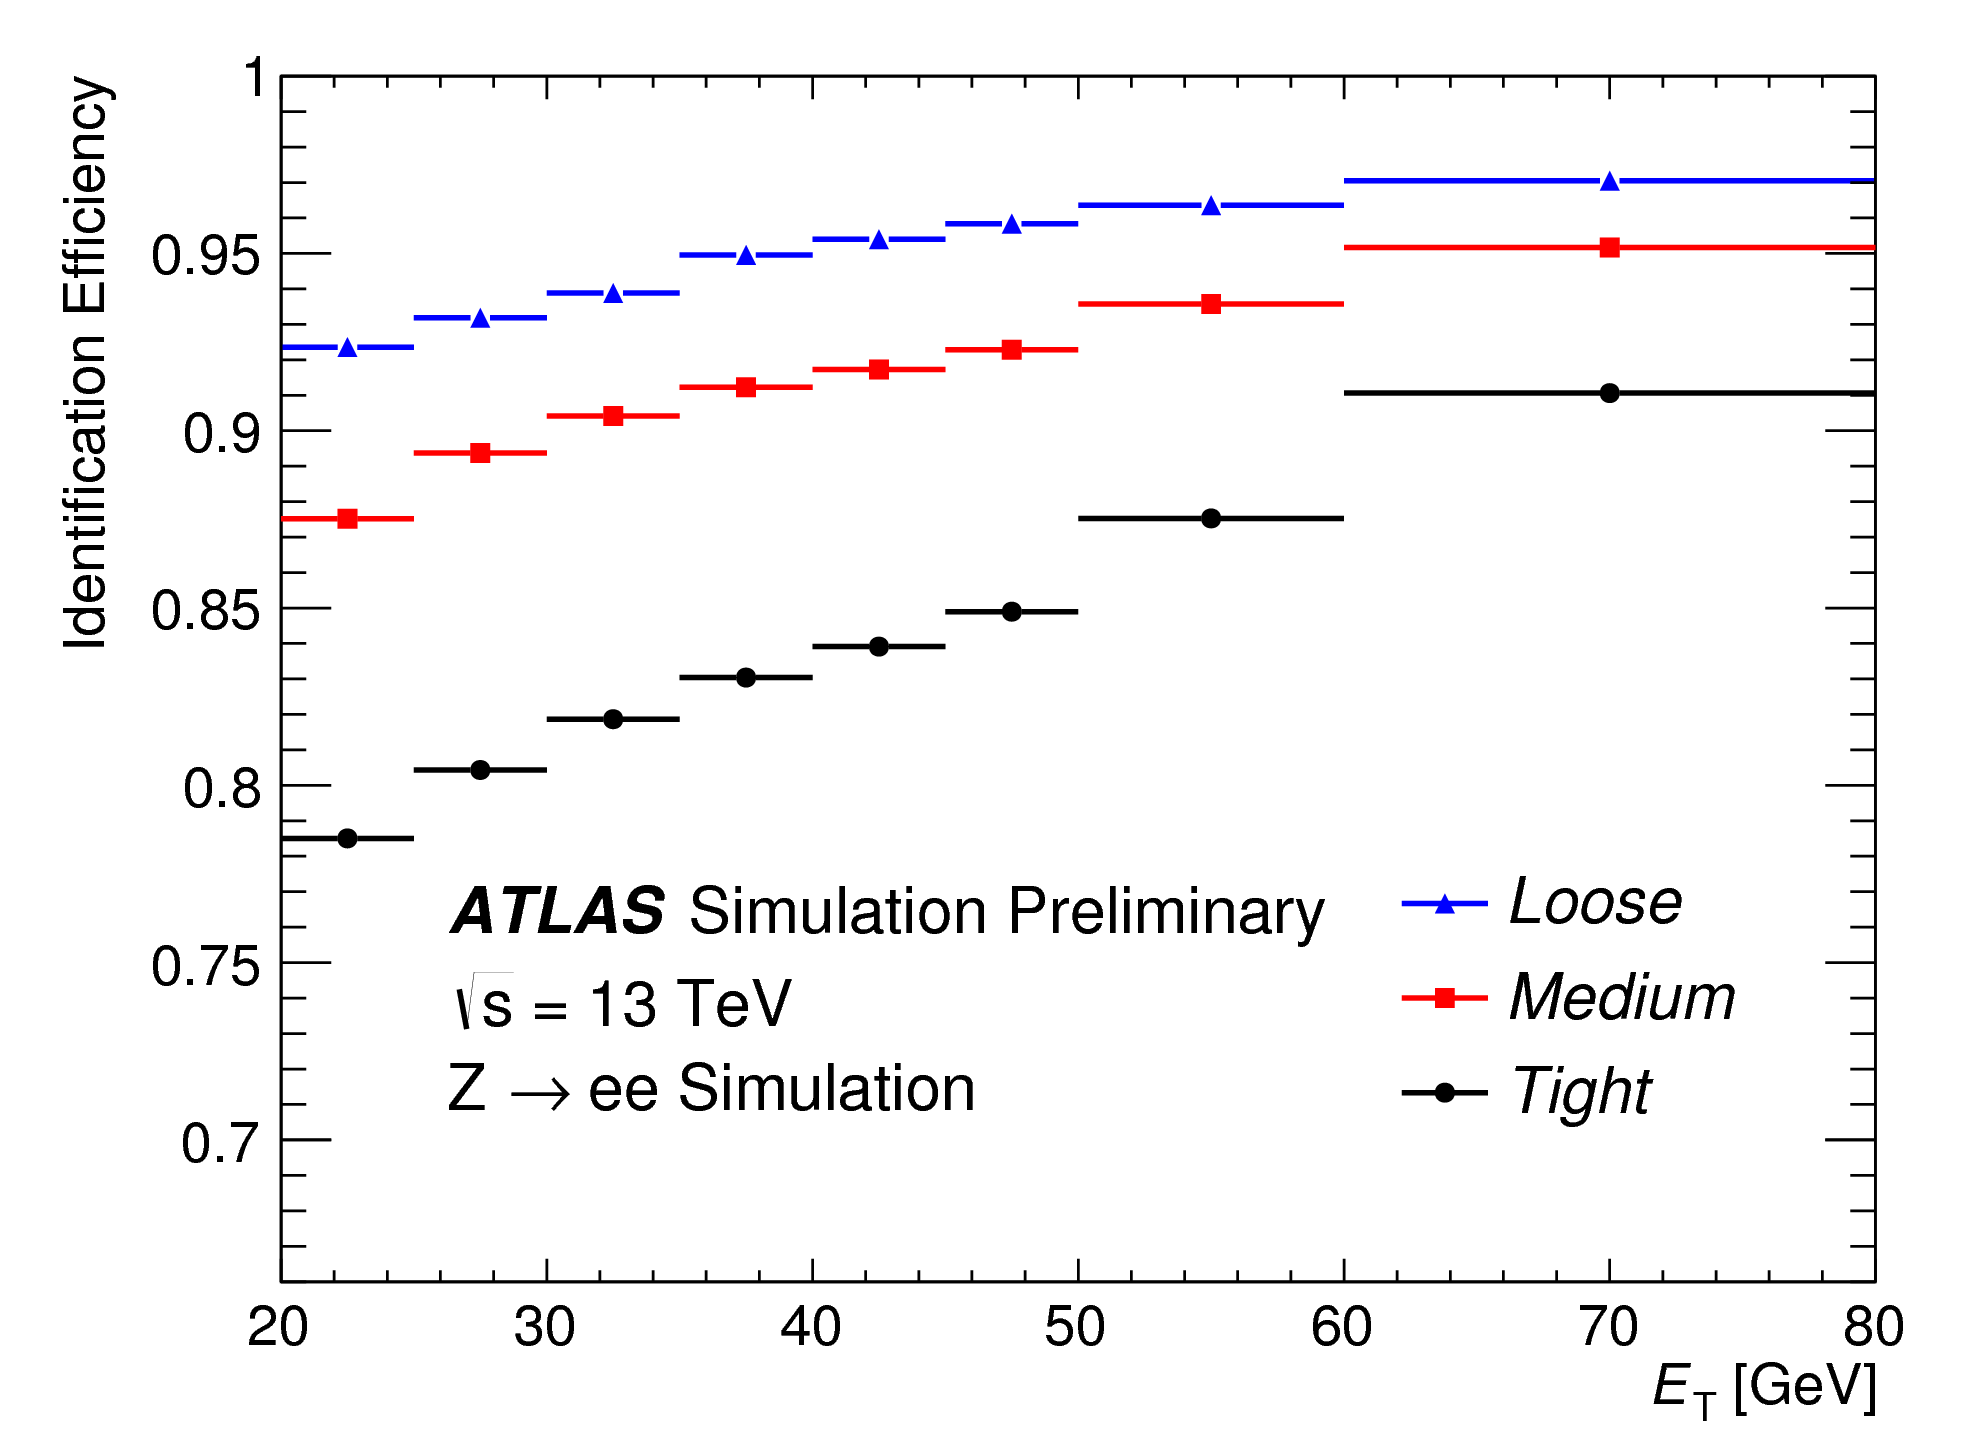
\includegraphics[width=.48\linewidth]{figures/reco/fig_01a.png}
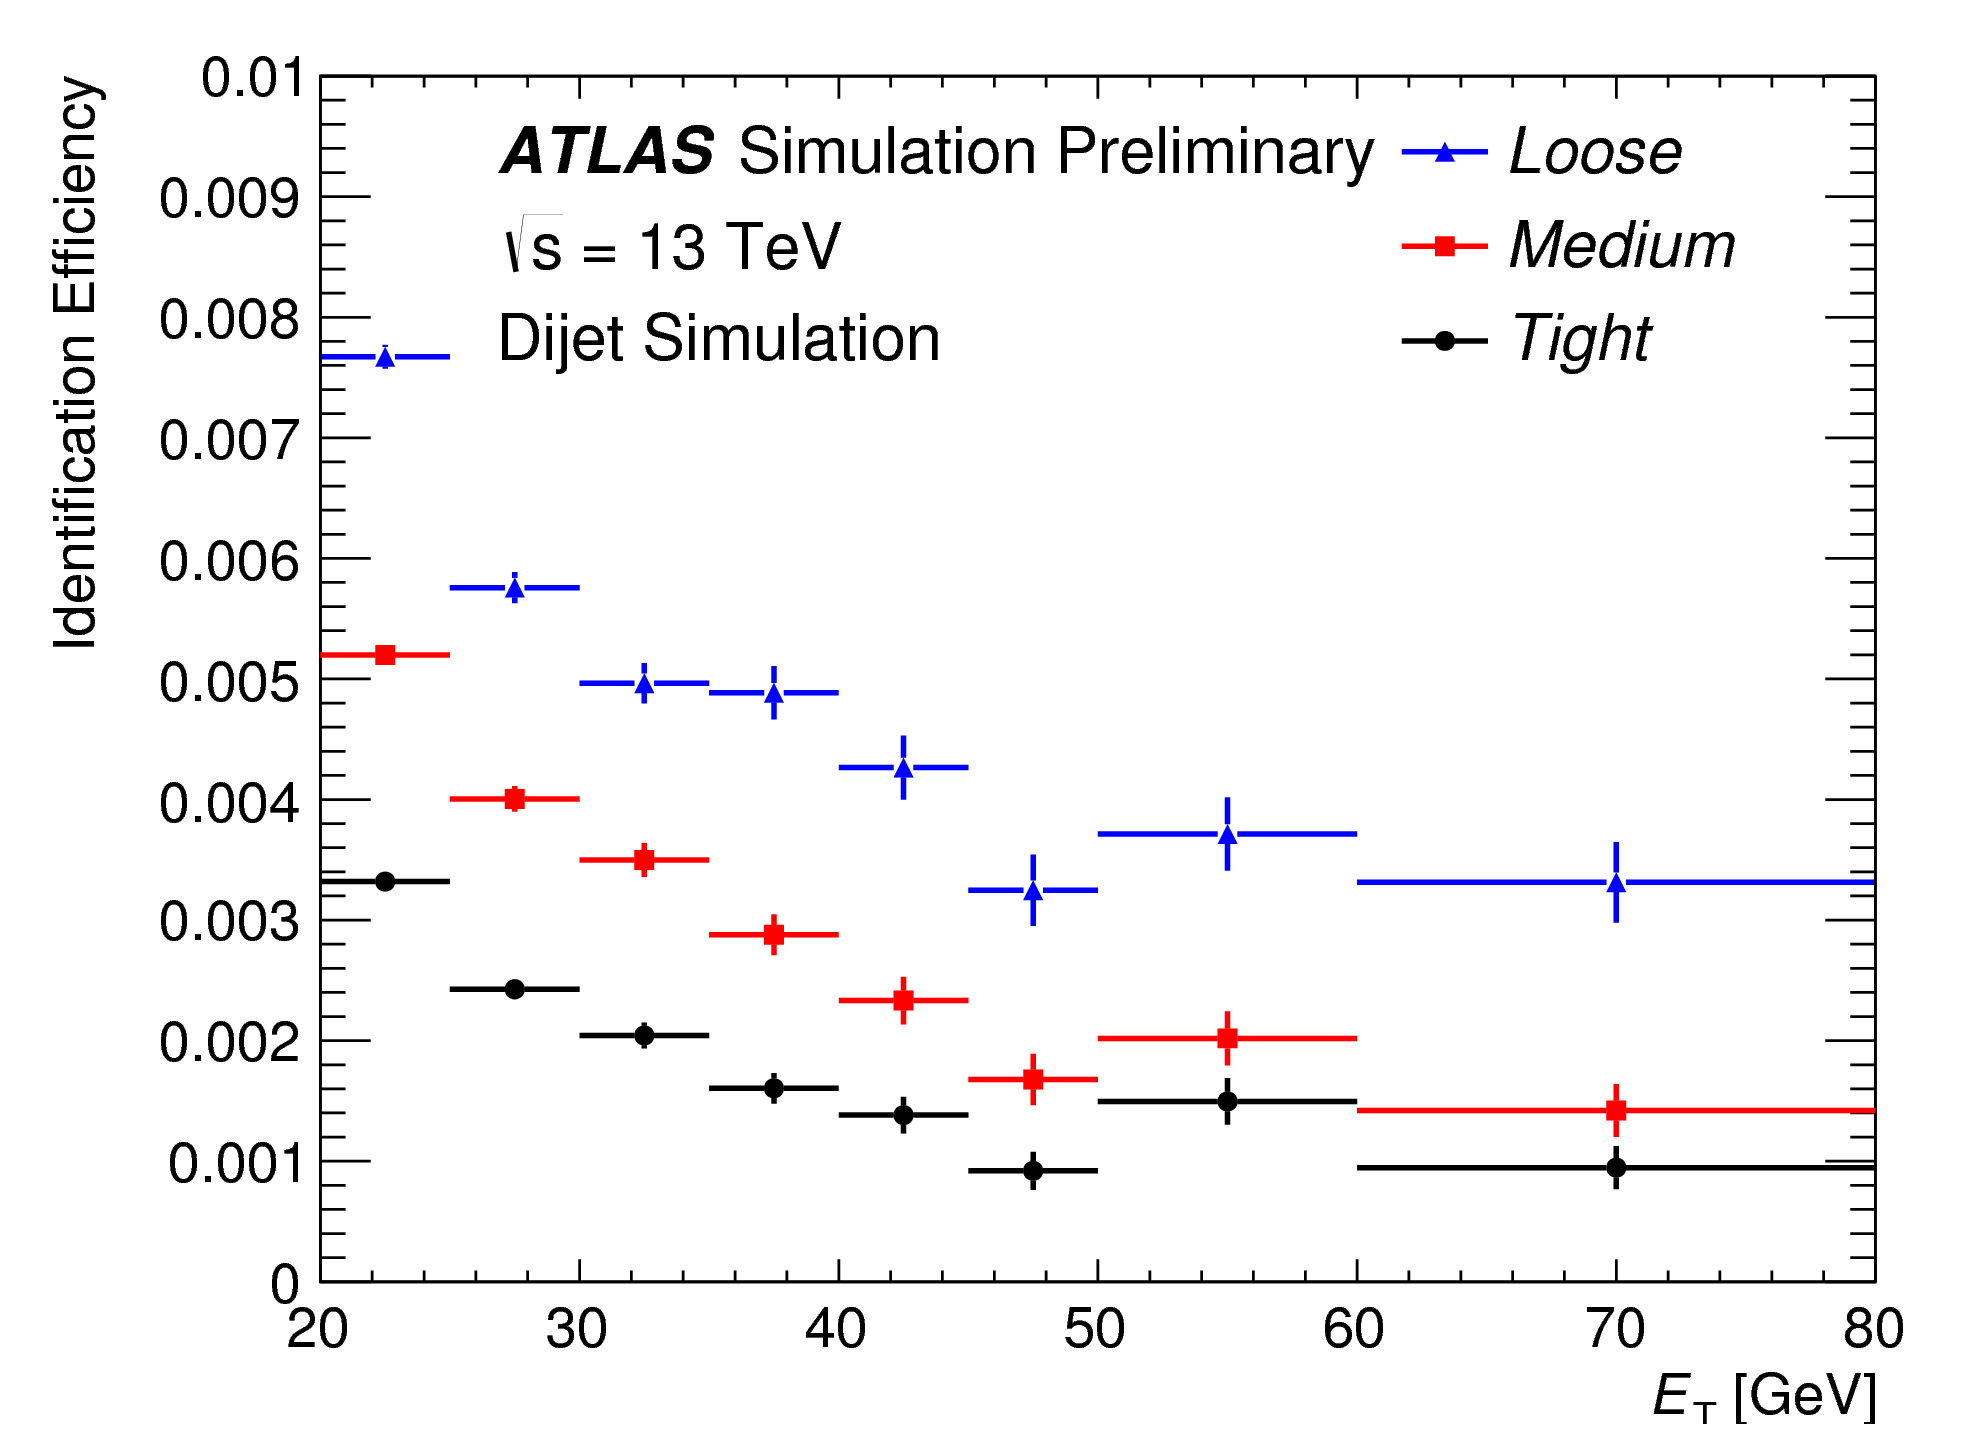
\includegraphics[width=.48\linewidth]{figures/reco/fig_01b.png}
\caption{ Identification efficiencies from \ac{MC} samples for \texttt{Loose}, \texttt{Medium}, and \texttt{Tight} working points. Left is the efficiency for identification of true electrons taken from $Z\rightarrow ee$ \ac{MC}, and right is the efficiency for mis-identification of jets as electrons taken from dijet \ac{MC} \cite{ATLAS-CONF-2016-024}.}
\label{fig:reco_el_eff}
\end{figure}
\end{centering}

\ac{MC} efficiencies can be compared to efficiencies measured in data to obtain a correction factor, which applied to \ac{MC} to better emulate the rates at which electrons are reconstructed and identified in data. \autoref{fig:reco_el_sf} shows a comparison of the combined reconstruction and identification efficiencies in data and \ac{MC}, with the resulting correction factors also displayed as the ratio. This analysis uses the \texttt{Medium} working point, which has correction factors ranging between 2 and 10\%. 

\begin{centering}
\begin{figure}[!hbt]
\myfloatalign
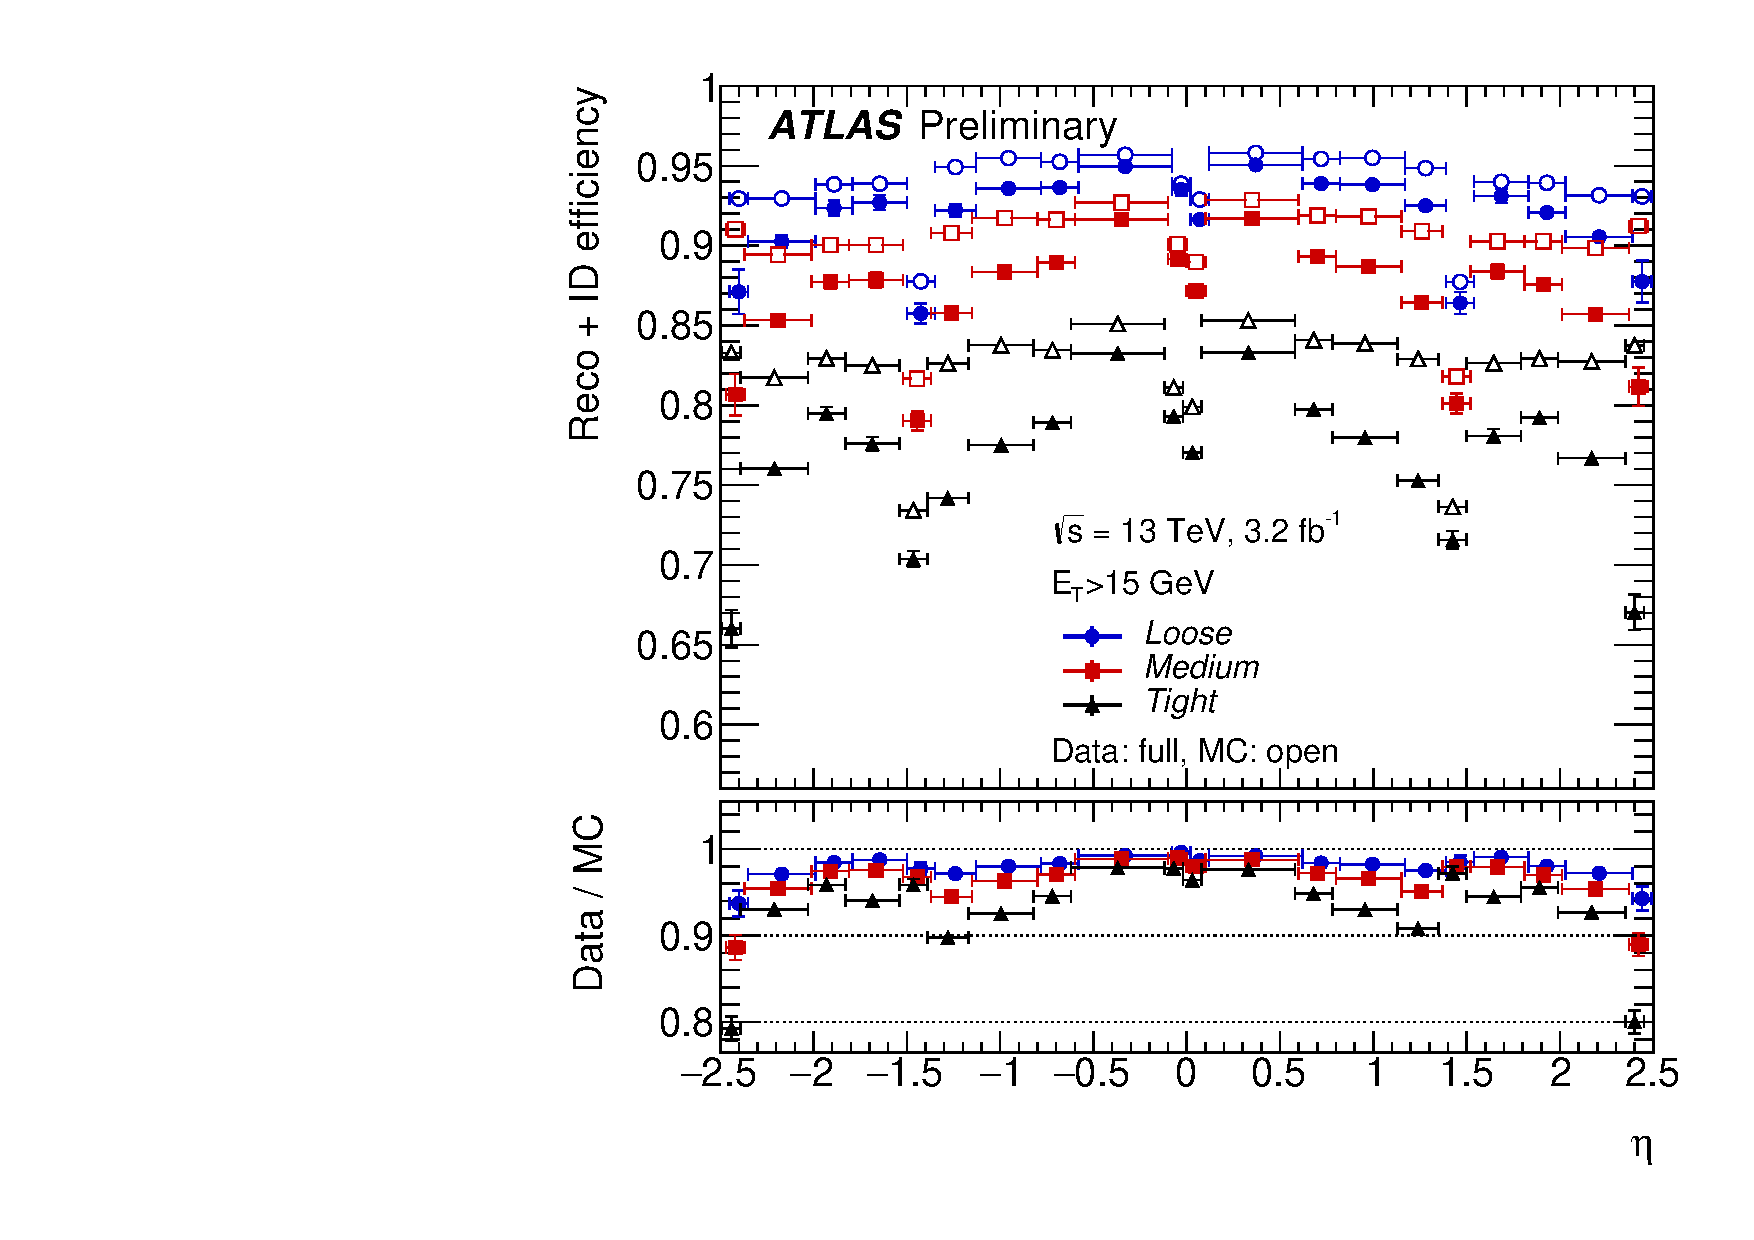
\includegraphics[width=.90\linewidth]{figures/reco/fig_14b.pdf}
\caption{ Combined electron reconstruction and identification efficiencies measured as a function of $\eta$ for data (using the tag-and-probe method on $Z\rightarrow ee$ events) and $Z\rightarrow ee$ \ac{MC}. Distributions include electrons with \et > 15 \gev. \cite{ATLAS-CONF-2016-024}.}
\label{fig:reco_el_sf}
\end{figure}
\end{centering}

Requirements are also made on electron \textit{isolation}, which quantifies the amount of energy deposited near the electron according calorimeter and track measurements. Isolation variables are primarily used to reject \textit{non-prompt} leptons, leptons which aren't produced by the initial hard scattering of the $pp$ collision. These can be produced by heavy flavor hadron decays and converted photons, as well as misidentified hadrons. Cuts are made on the amount of nearby calorimetric energy and sum of the \pt of any nearby tracks relative to the electron's energy, forming a series of working points. Working points are created based on their efficiency, including \texttt{Tight} and \texttt{Loose} working points, which operate at 95 and 98\% efficiency respectively. The most effective working points target different efficiencies as a function of \pt, with higher efficiencies possible at high \pt due to reduced fake backgrounds. There are two such working points, \texttt{Gradient} and \texttt{GradientLoose}. They each have a 99\% efficiency for electrons with \pt > 60 \gev, but 90 and 95\% efficiencies at 25 \gev. To recover the largest possible fraction of electrons, this analysis uses \texttt{GradientLoose}.

\section{Photons}
\label{sec:reco_photons}

The reconstruction of photons is performed in parallel to electron reconstruction. Seed clustering is performed, and tracks are matched to these clusters, as in the case of the electron reconstruction described in \autoref{sec:reco_electrons}. 

Photons can be converted to electron-positron pairs in the \ac{ID}, leaving a pair of tracks, or they can pass through without conversion, leaving no tracks behind. As a consequence, calorimeter clusters resulting from photons can have no tracks associated with them, two tracks, or one track, in the case that one of the conversion tracks is not reconstructed. The reconstruction software attempts to identify all these scenarios and differentiate these clusters from electron and hadron deposits \cite{1606.01813}.

Two-track clusters are required to consist of two oppositely charged tracks that emerge from a conversion vertex running parallel to one another. A likelihood that these tracks are from electrons is determined using the high threshold hits in the \ac{TRT}, and quality requirements are made on the tracks using this likelihood. For tracks with silicon hits, a loose likelihood requirement of 10\% is made, while tracks without silicon hits are required to have at least 80\% likelihood. The tracks are then fit to determine the conversion vertex, and quality cuts are made, such as requiring that conversion vertices within the silicon volume correspond to tracks with silicon hits. 

Single track clusters occur most often from conversions in the outermost layers of the \ac{ID}, and are more difficult to reconstruct. Tracks are typically lost because an electron or positron resulting from the conversion has a \pt too low to be reconstructed, or because the two tracks are so close together that they're identified as a single track. The single track is required to have at least a 95\% electron likelihood from \ac{TRT} hits, and must not have a hit in the innermost layer of the Pixel Detector. The conversion vertex is defined as the first hit of the single track. 

The tracks associated with these conversion vertices are extrapolated to the calorimeter and matched to cluster, except in the case that there are two tracks that differ substantially in their \pt measurements, in which case the position of the conversion vertex is used for extrapolation to the calorimeter, assuming a straight-line trajectory. If multiple vertices are matched to a single cluster, preference is given to vertices with double tracks, silicon hits, and finally to tracks closest to the interaction point. 

Any cluster with neither a conversion vertex or a track associated with it is identified as an unconverted photon. Clusters associated with both electrons and photons are assigned to one or the other based on their properties. Clusters are preferentially identified as photons in the case that they are matched to a conversion vertex in which at least one track is associated with both the vertex and the cluster, or if the associated tracks have a \pt smaller than the cluster's \pt. $E/p$, the ratio of the cluster and track energy measurements, can also be used to differentiate electrons and photons. Electron candidates are instead reconstructed as photons if they have $E/p>10$ or if the track matched to the electron has \pt below 2 \gev. 


Photon energy is determined in a 3$\times$5 (3$\times$7) window for unconverted (converted) photons in the barrel, where the window is expanded to compensate for the increased spread of energy from the conversion products. In the endcap, the 5$\times$5 window is used in all cases. Like the electrons, the calibration of the photon's energy accounts for energy loss before the calorimeter, as well as energy deposited outside the cell and beyond the electromagnetic calorimeter.

Photon identification is performed in the range $|\eta|<2.37$ using a series of cuts on the shape of the shower in the electromagnetic calorimeter, as well as the amount of additional energy deposited in the hadronic calorimeter. Photons in the the so called \textit{crack} region of the calorimeter ($1.37<|\eta|<1.52$), where a discontinuity prevents accurate assessment of photon energy, are rejected. The photon identification has only one working point, called \texttt{Tight}, which has an identification efficiency of 53–64\%(47–61\%) for unconverted (converted) photons with \et = 10 \gev~and 88–92\% (96–98\%) for photons with \et $\geq$ 100 \gev~\cite{ATL-PHYS-PUB-2016-014}. Efficincies as a function of \pt measured in the 2016 data and compared to \ac{MC} can be seen in \autoref{fig:reco_photon_eff}.

\begin{centering}
\begin{figure}[!hbt]
\myfloatalign
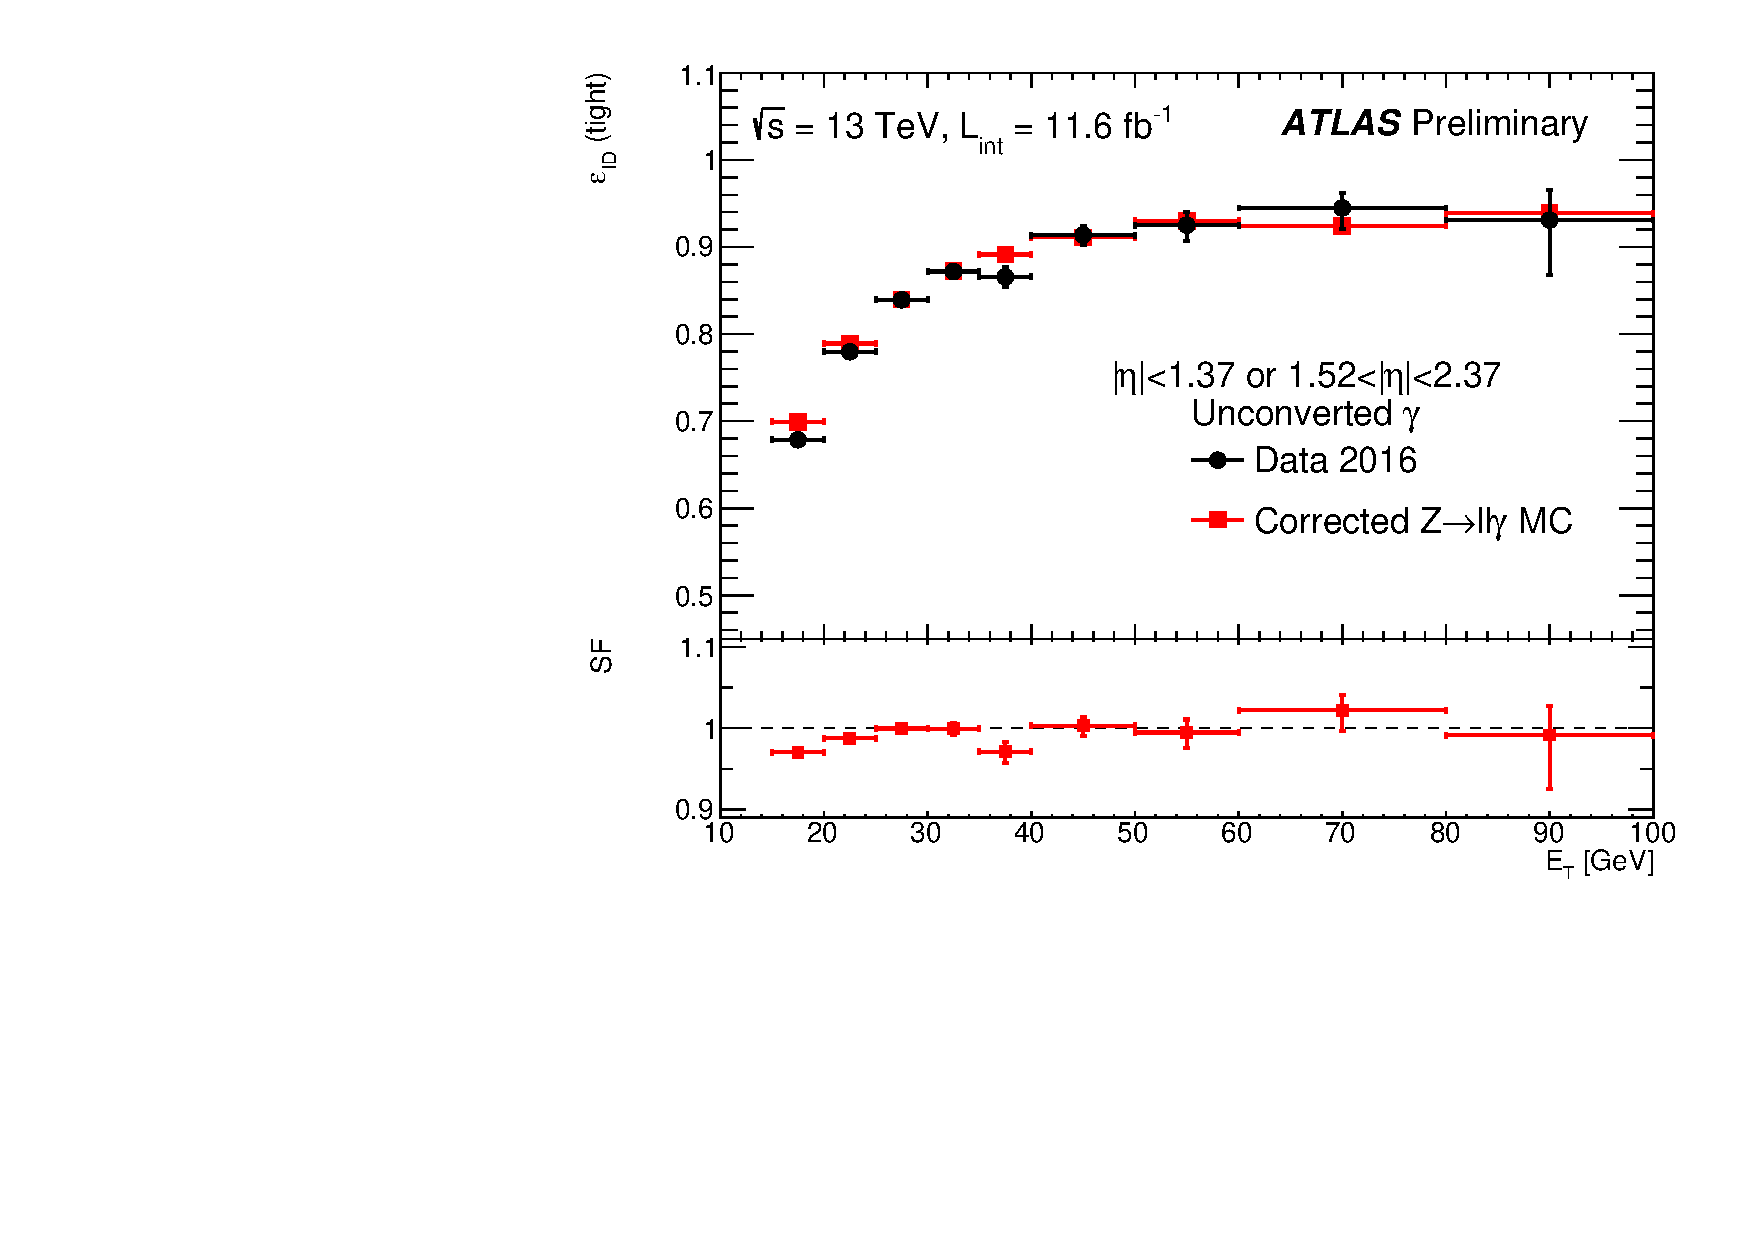
\includegraphics[width=.48\linewidth]{figures/reco/photon_fig_01.pdf}
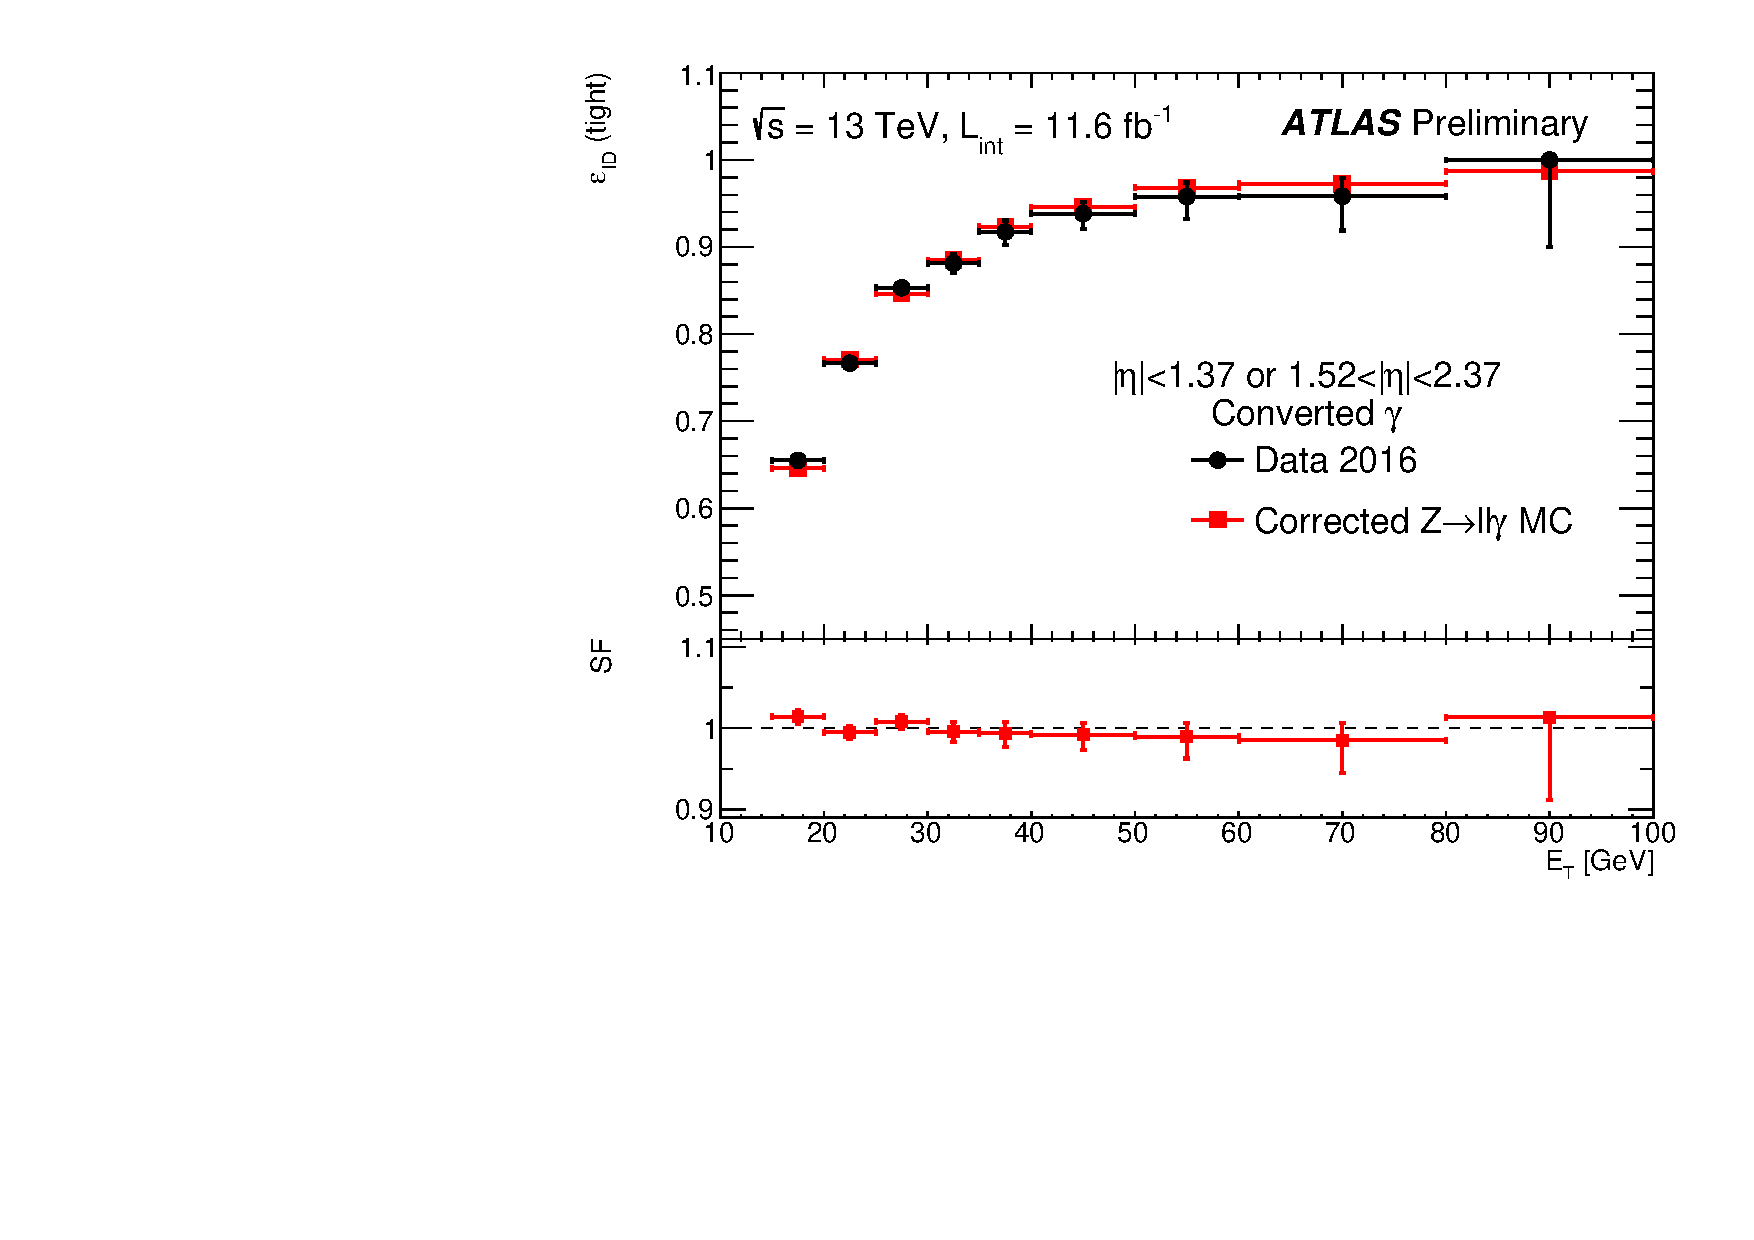
\includegraphics[width=.48\linewidth]{figures/reco/photon_fig_02.pdf}
\caption{ Comparison of \texttt{Tight} identification efficiency measurements from data and $Z\rightarrow \ell\ell\gamma$ \ac{MC} for unconverted (left) and converted (right) photons, with an inclusive $\eta$ selection. The bottom of each figure shows the ratio of data and \ac{MC} efficiencies. \cite{EGAM-2016-003}.}
\label{fig:reco_photon_eff}
\end{figure}
\end{centering}

Photon isolation, like electron isolation, can be determined as the combination of nearby calorimeter deposits and tracks. Fixed cuts on the isolation as a fraction of photon energy is typically used. A working point called \texttt{FixedCutTight} reconstructs the amount of calorimeter energy (excluding that of the photon) in a cone of $\Delta R  = 0.4$ around the photon and the amount of energy from the sum of track \pt in a cone of $\Delta R = 0.2$, including only tracks associated with the primary vertex. Defined relative to the photon's \pt, this working point includes photons with calorimetric isolation less than 0.022 \pt + 2.45 \gev~and track isolation less than 0.05 \pt \cite{isolation}. 

\section{Muons}
\label{sec:reco_muons}

Muon reconstruction is performed independently in the \ac{ID} and the \ac{MS}, then the two measurements are combined when consistent tracks are found in each system \cite{1603.05598}. The \ac{ID} reconstruction is performed using the tracking algorithms described in \autoref{sec:tracking}, and includes tracks with $|\eta|<2.5$. 

The \ac{MS} track reconstruction is performed in the $|\eta|<2.7$ range and begins with a search in each muon chamber for patterns of hits consistent with a track, called \textit{segments}. The \ac{MDT} chamber hits are fit to a straight line, and nearby \ac{RPC} and \ac{TGC} chambers provide the coordinate orthogonal to the magnetic curvature for these hits. Segments are also built in the \ac{CSC}, where they are required to be loosely consistent with a track originating from the interaction point. 

These segments are then fit together, starting from the middle layers of the \ac{MS}, with track quality requirements on the resulting combinations based on the $\chi^2$ of the fits. Tracks must have at least two segments, except in the transition region between the barrel and endcap, where a single segment can qualify as a track. Segments are allowed to be shared between multiple tracks in the initial reconstruction, but after the combination, tracks with shared segments and poor $\chi^2$ are removed.    

These \ac{MS} tracks are then combined with measurements from the \ac{ID} and calorimeters. The best quality muons are combined muons, which have \ac{ID} and \ac{MS} tracks associated to them, the hits of which are re-fit to form a combined track. \ac{MS} hits can be added or removed at this stage based on their consistency with the new track. Lower quality muon candidates are also defined. Extrapolated muons have only \ac{MS} tracks and their trajectories are required to be consistent with the interaction point. Calorimeter-tagged muons combine an \ac{ID} track with a calorimeter deposit consistent with a muon, while segment-tagged muons combine an \ac{ID} track with a segment in the \ac{MS}. Muons with shared \ac{ID} tracks are not allowed, with preference given to combined muons, then calorimeter-tagged muons, and lastly segment-tagged muons. 

There are four muon identification working points for muons: \texttt{Loose}, \texttt{Medium}, \texttt{Tight}, and \texttt{High-p$_\texttt{T}$}. These working points all have different efficiencies for the identification of muons, balanced against the mis-identification of hadrons. One of the key variables for their discrimination is $q/p$ significance, which quantifies the consistency between the \ac{ID} and \ac{MS} measurements of momentum. The $\chi^2$ of the combined fit is also an important discriminator. 

The \texttt{Loose}, \texttt{Medium}, and \texttt{Tight} selections are inclusive, with all \texttt{Tight} muons passing the \texttt{Medium} requirements, and \texttt{Medium} muons passing the \texttt{Loose} requirements. %The \texttt{Loose} requirement includes all types of reconstructed muons, but allows muons without \ac{MS} tracks (calorimeter- and segment-tagged muons) only in the $\eta<0.1$ range where there is a gap in the \ac{MS} coverage to accommodate cabling for the calorimeter system. 
The \texttt{Medium} working point includes only combined and extrapolated muons, and is the default for most \ac{ATLAS} analyses, including this one. Extrapolated muons are allowed only outside the \ac{ID} tracking system ($|\eta|>2.5$) for this working point, but this region is excluded by this analysis because of the decreased efficiency and larger \pt resolution of these muons. As a consequence, this analysis uses only combined muons. For these muons, the \texttt{Medium} working point requires at least three hits in at least two \ac{MDT} layers (except in the $\eta<0.1$ region) and a $q/p$ significance cut is made to reduce backgrounds. Due to the lack of coverage at low $\eta$, there is a drop in efficiency in this region, as shown in \autoref{fig:reco_muon_eta}. %The \texttt{Tight} working point additionally cuts on $\chi^2$ and makes further requirements on the consistency between \ac{ID} and \ac{MS} \pt measurements. 

\begin{centering}
\begin{figure}[!hbt]
\myfloatalign
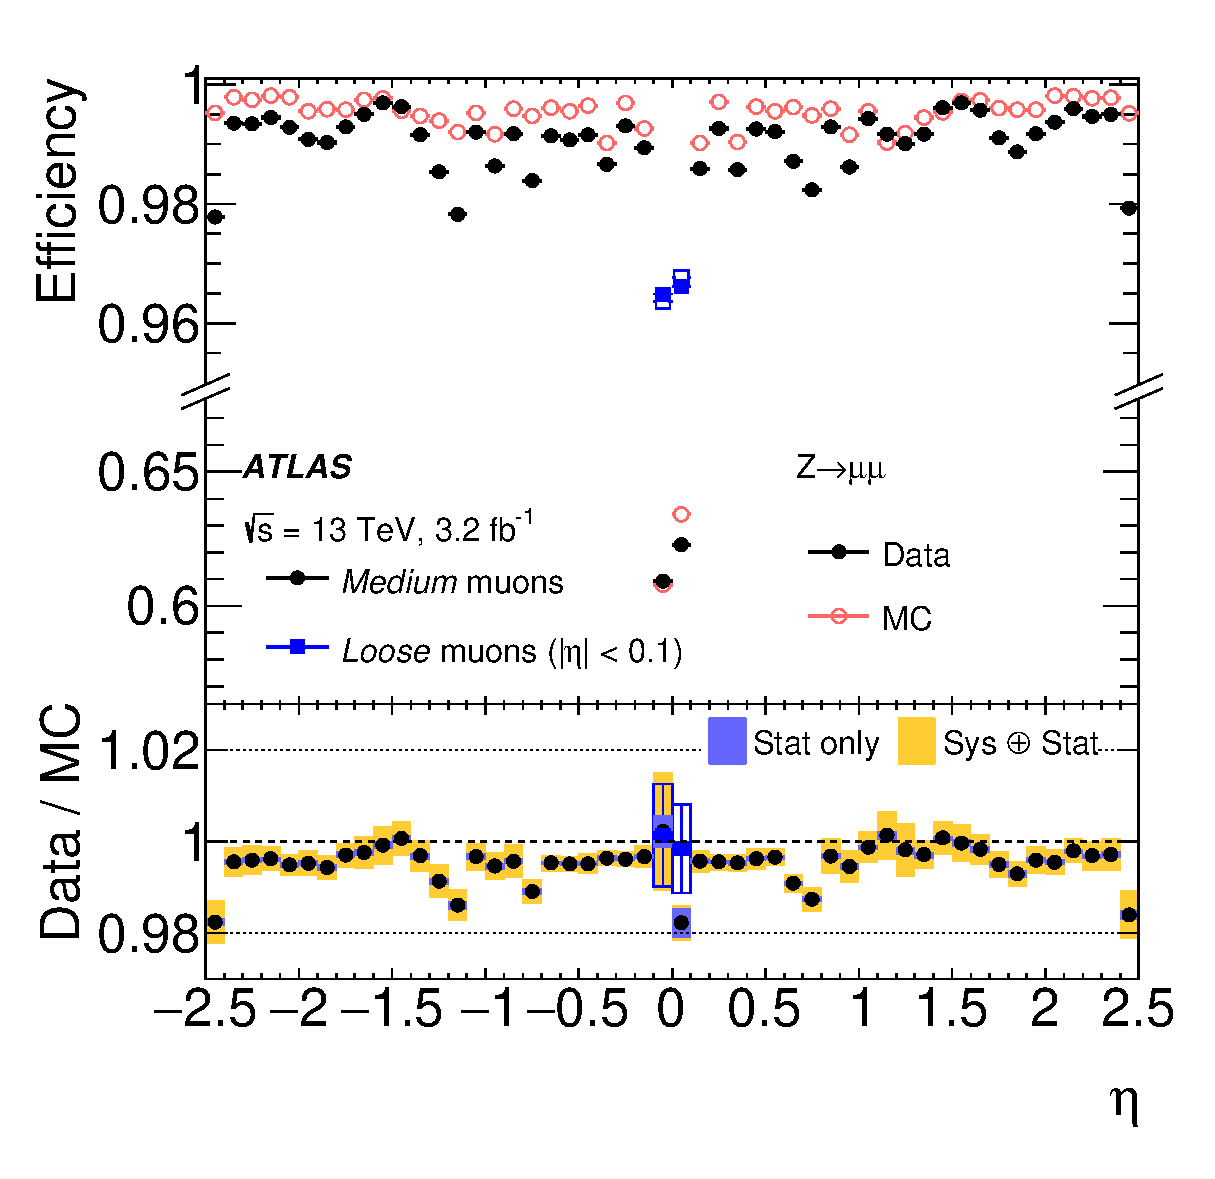
\includegraphics[width=.9\linewidth]{figures/reco/fig_03a.eps}
\caption{Muon reconstruction efficiency for the \texttt{Medium} and \texttt{Loose} working points measured with $Z\rightarrow\mu\mu$ events in data and in \ac{MC} as a function of $\eta$. The ratio between the two is shown at the bottom. The \texttt{Loose} working point efficiency is shown only at  small $|\eta|$, where the loosened requirements cause the largest difference from the \texttt{Medium} working point \cite{1603.05598}. }
\label{fig:reco_muon_eta}
\end{figure}
\end{centering}

The \texttt{High-p$_\texttt{T}$} working point is designed to minimize the resolution for high-\pt muons, at the cost of lower efficiencies. Muons passing the \texttt{High-p$_\texttt{T}$} requirements must have at least three \ac{MDT} hits in three layers, which decreases efficiency but gives greatly improved \pt resolution. In addition, some regions of the \ac{MS} with poor alignment are vetoed to cut down on mismeasurement. Compared to the default working point these muons have much lower efficiency: 78\% (90\%) for \texttt{High-p$_\texttt{T}$} muons compared to 96\% (96\%) for \texttt{Medium} in the \pt range of 4-20 \gev~(20-100 \gev). The efficiency as a function of $\eta$ for this working point can be seen in \autoref{fig:reco_muon_eta_highpt}, where the efficiency loss due to the of vetoing of some chambers is especially apparent. Mismodeling of the alignment and the specificity of the momentum resolution cuts cause a large discrepancy between data and \ac{MC} efficiencies, resulting in scale factors that differ from unity by as much as 10\%. This working point was considered for this analysis, where mismeasurement of muons increases \ac{SM} backgrounds, but ultimately the \texttt{Medium} working point was chosen for its superior efficiency and better modeling in \ac{MC}.

\begin{centering}
\begin{figure}[!hbt]
\myfloatalign
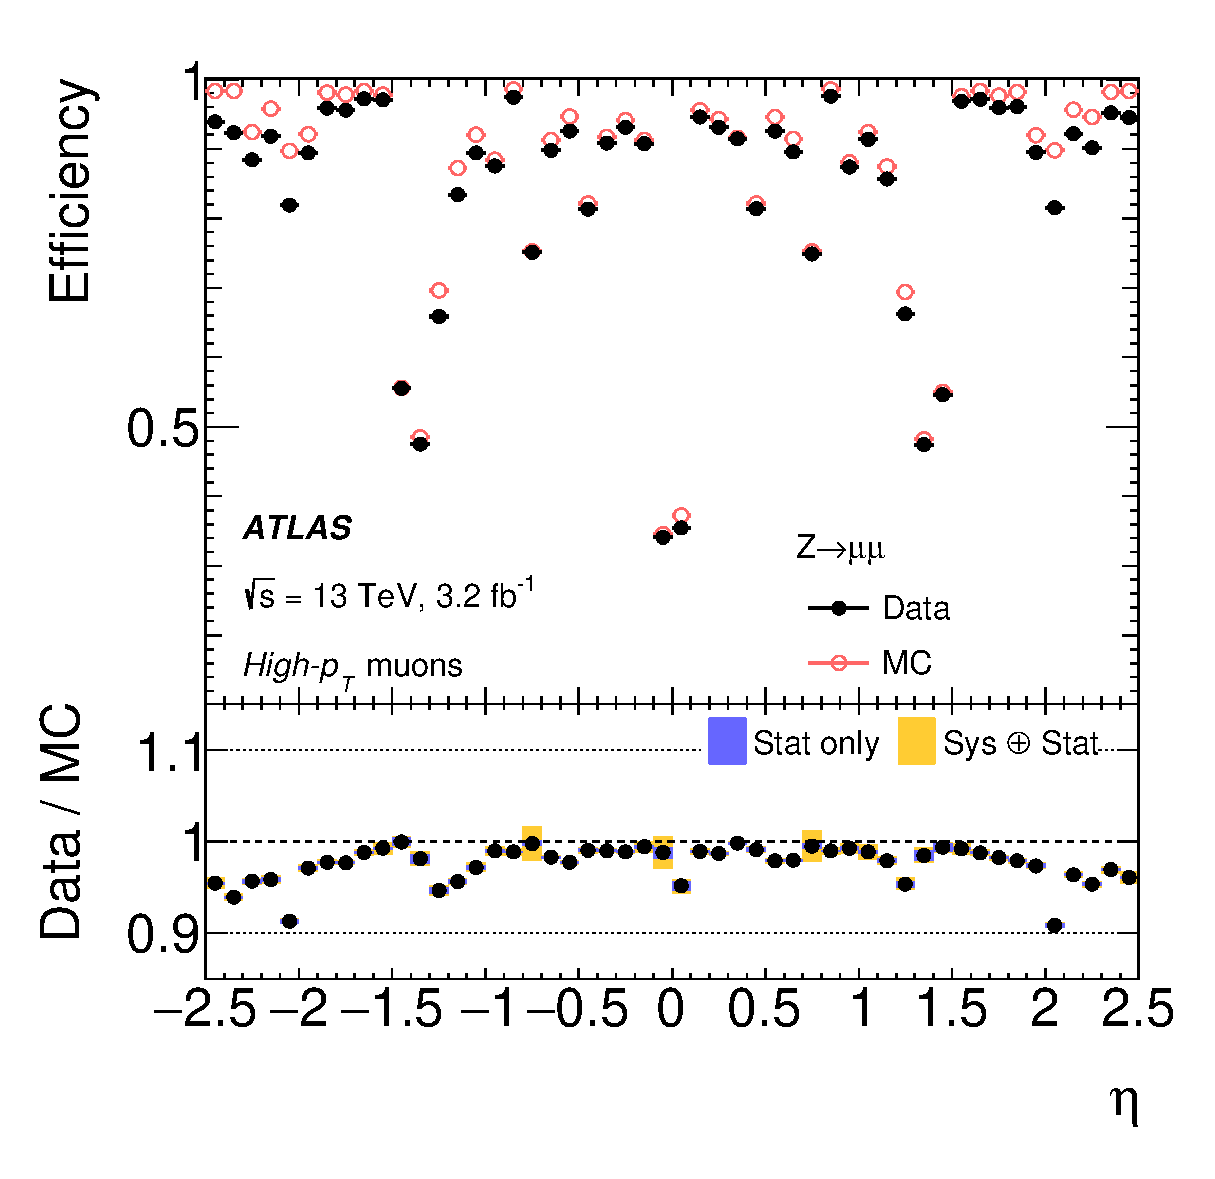
\includegraphics[width=.9\linewidth]{figures/reco/fig_03c.eps}
\caption{Muon reconstruction efficiency for the \texttt{High-p$_\texttt{T}$} working point measured with $Z\rightarrow\mu\mu$ events in data and in \ac{MC} as a function of $\eta$. The ratio between the two is shown at the bottom. \cite{1603.05598} }
\label{fig:reco_muon_eta_highpt}
\end{figure}
\end{centering}

The isolation selection for muons is designed in the same way as the electron isolation, and also called \texttt{GradientLoose}. This working point makes cuts on a combination of nearby calorimeter- and track-based energy measurements, with an increasing efficiency as a function of \pt. The \texttt{GradientLoose} working point is constructed such that muons with \pt of 25 \gev~have an efficiency of 95\%, and muons with \pt of 60 \gev~have an efficiency of 99\%. 

\section{Jets}
\label{sec:reco_jets}

Jets are the most complicated objects to reconstruct in the \ac{ATLAS} detector because each jet is an assembly of many hadronic particles. In contrast to a lepton, whose reconstructed energy can easily be compared to its true energy from simulation, even a jet's true energy is ambiguous, and is dependent on the choice of the jet's definition. The standard jet reconstruction algorithm used in the \ac{ATLAS} experiment is called anti-$k_t$ \cite{Cacciari:2008gp}. 

This algorithm begins with clusters in the calorimeter defined by topologically connected cells with energy deposits significantly higher than the noise background. There are two collections used most commonly for analysis. One uses cluster energies calibrated for electromagnetic showers (\acs{EM}), and another uses clusters calibrated to the energies of hadronic showers. The second uses a method called \ac{LCW}, which first determines the extent to which the cluster is electromagnetic or hadronic based on the energy density and the shower depth, then applies a calibration accordingly for each cluster.

To reconstruct jets, a set of clusters is chosen and the anti-$k_t$ algorithm is then applied. These clusters are grouped together according to the distance measure
%
\begin{equation}
d_{ij} = \mathrm{min}(k^{-2}_{ti}, k^{-2}_{tj}) \frac{\Delta_{ij}^2}{R^2}
\end{equation}
%
where $R$ is the algorithm's radius parameter, typically set to 0.4, $\Delta$ gives the angular separation of the two clusters, and $k_t$ is the transverse momentum associated with the cluster. 

The grouping process begins with each cluster as a \textit{pseudo-jet}, with its axis and \pt is determined as if it were a typical jet. Then, the pair of pseudo-jets with the smallest $d_{ij}$ are grouped together, forming a new pseudo-jet, and its axis and \pt are reassessed. This grouping continues until there is a pseudo-jet with \pt smaller than the $d_{ij}$ of any pseudo-jet pair, at which point this pseudo-jet becomes a jet, and is removed from the collection. The clustering process continues until all clusters are associated with a jet. 

The inverse dependence on the $k_t$ of the cluster produces jets with energetic cores and softer edges, which matches the expectation from a hadronic shower. In addition it is infrared and collinear safe, with neither soft emission nor collinear particles altering the reconstruction of the jet.

A series of calibrations are then applied to these jets. The first is to correct for additional hadronic energy due to pile-up. \autoref{fig:reco_jet_nvtx} demonstrates the impact of pile-up on the energy density of an event. The energy density of each jet is defined as the jet's \pt divided by the its area, and the overall event's energy density is defined as the median value of this quantity for jets with \pt > 20 \gev. In events with high numbers of primary vertices, the resulting high energy density can affect the amount of stray energy associated with reconstructed jets. To remove the bias on jet energy measurements that results from multiple primary vertices, a correction factor is determined using \ac{MC}. It is parametrized in terms \pt, $\eta$, and the number of primary vertices in the event, as well as the average number of interactions per event in the event's luminosity block, which makes correction for out-of-time pile-up possible. Next, jets are corrected to have their origin at the primary vertex instead of the center of the \ac{ATLAS} detector. After that, the jets are corrected based on $\eta$ dependent \acf{JES} factors derived from data and \ac{MC} independently. \autoref{fig:reco_JES} shows the energy response, the inverse of these factors, for \ac{EM} jets. Lastly, an observed bias in the $\eta$ measurement of jets is accounted for. 

\begin{centering}
\begin{figure}[!hbt]
\myfloatalign
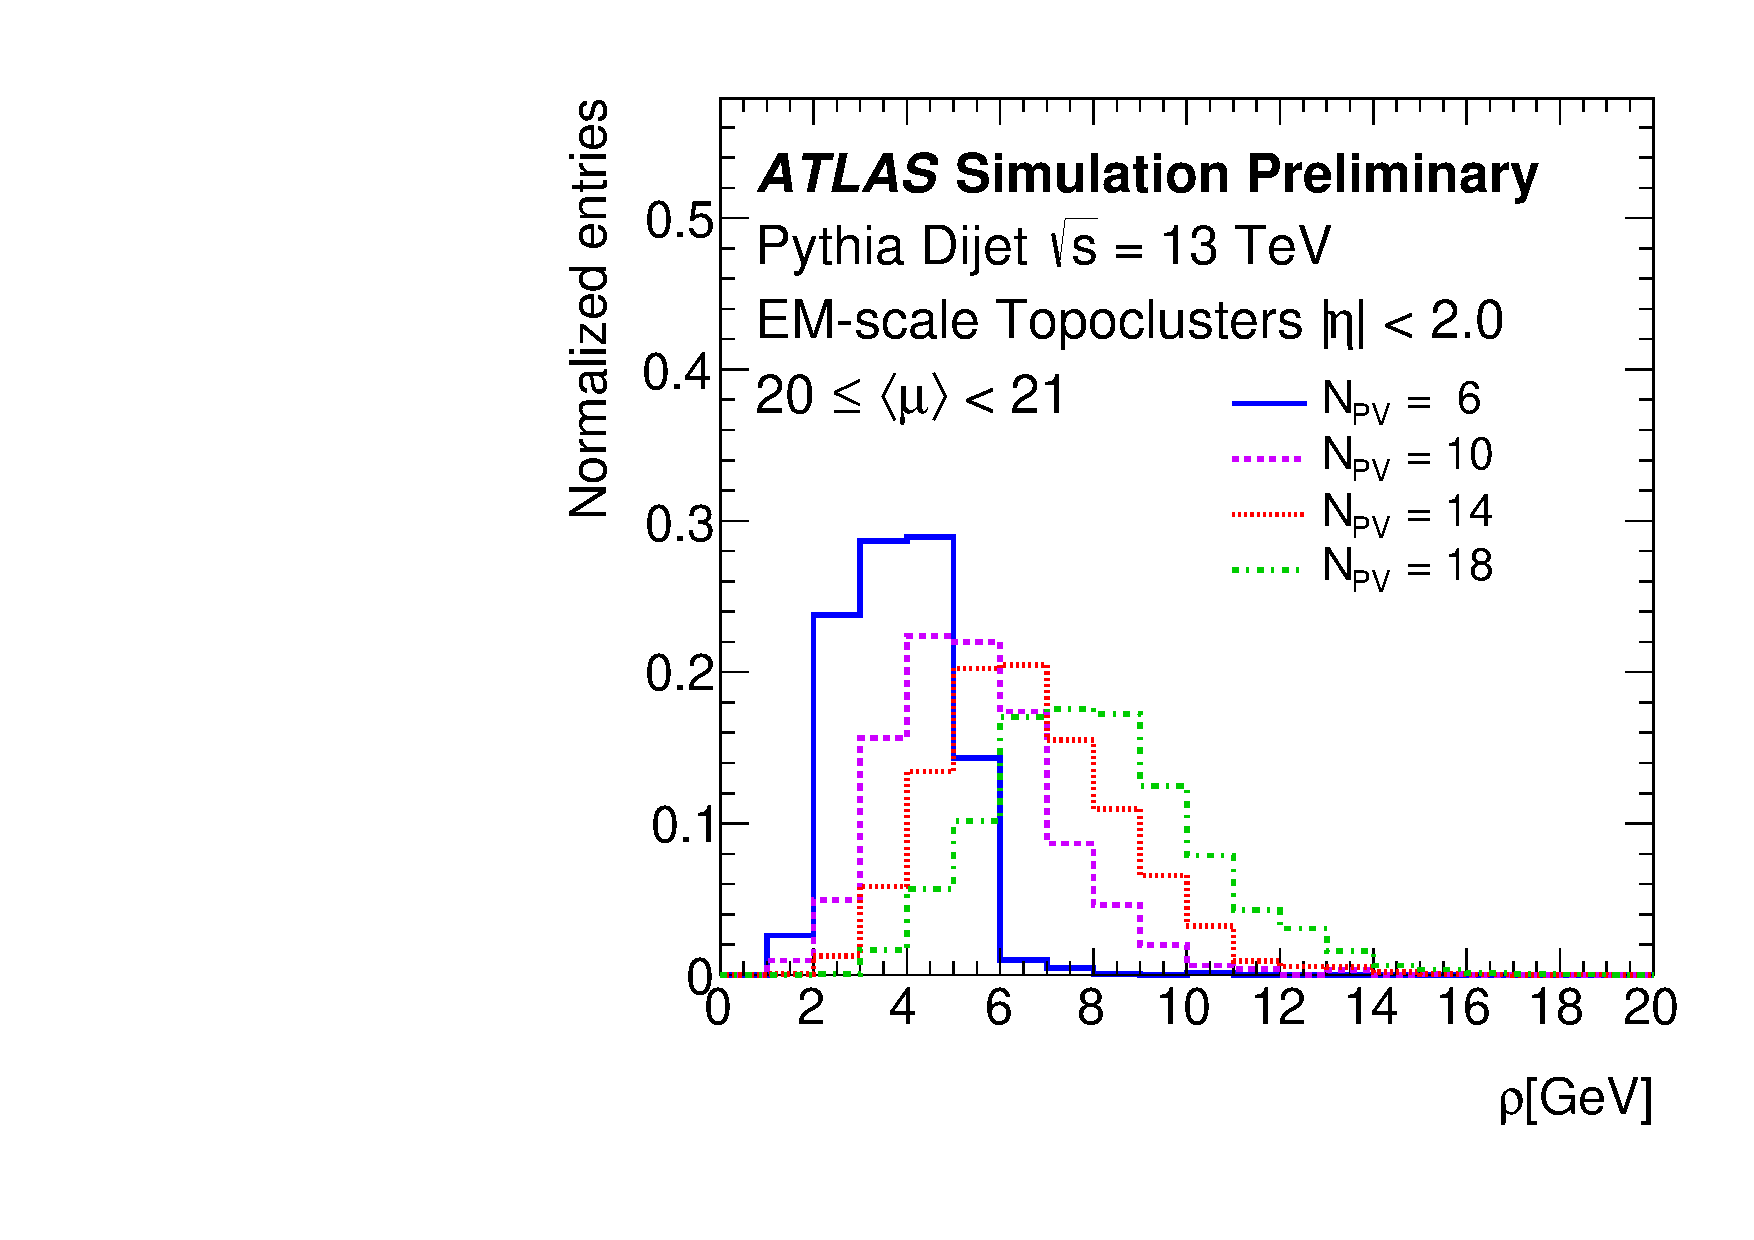
\includegraphics[width=.9\linewidth]{figures/reco/fig_02.pdf}
\caption{ Distribution of event \pt density, $\rho$, taken from \ac{MC} dijets for different numbers of primary vertices. \cite{ATL-PHYS-PUB-2015-015} }
\label{fig:reco_jet_nvtx}
\end{figure}
\end{centering}

\begin{centering}
\begin{figure}[!hbt]
\myfloatalign
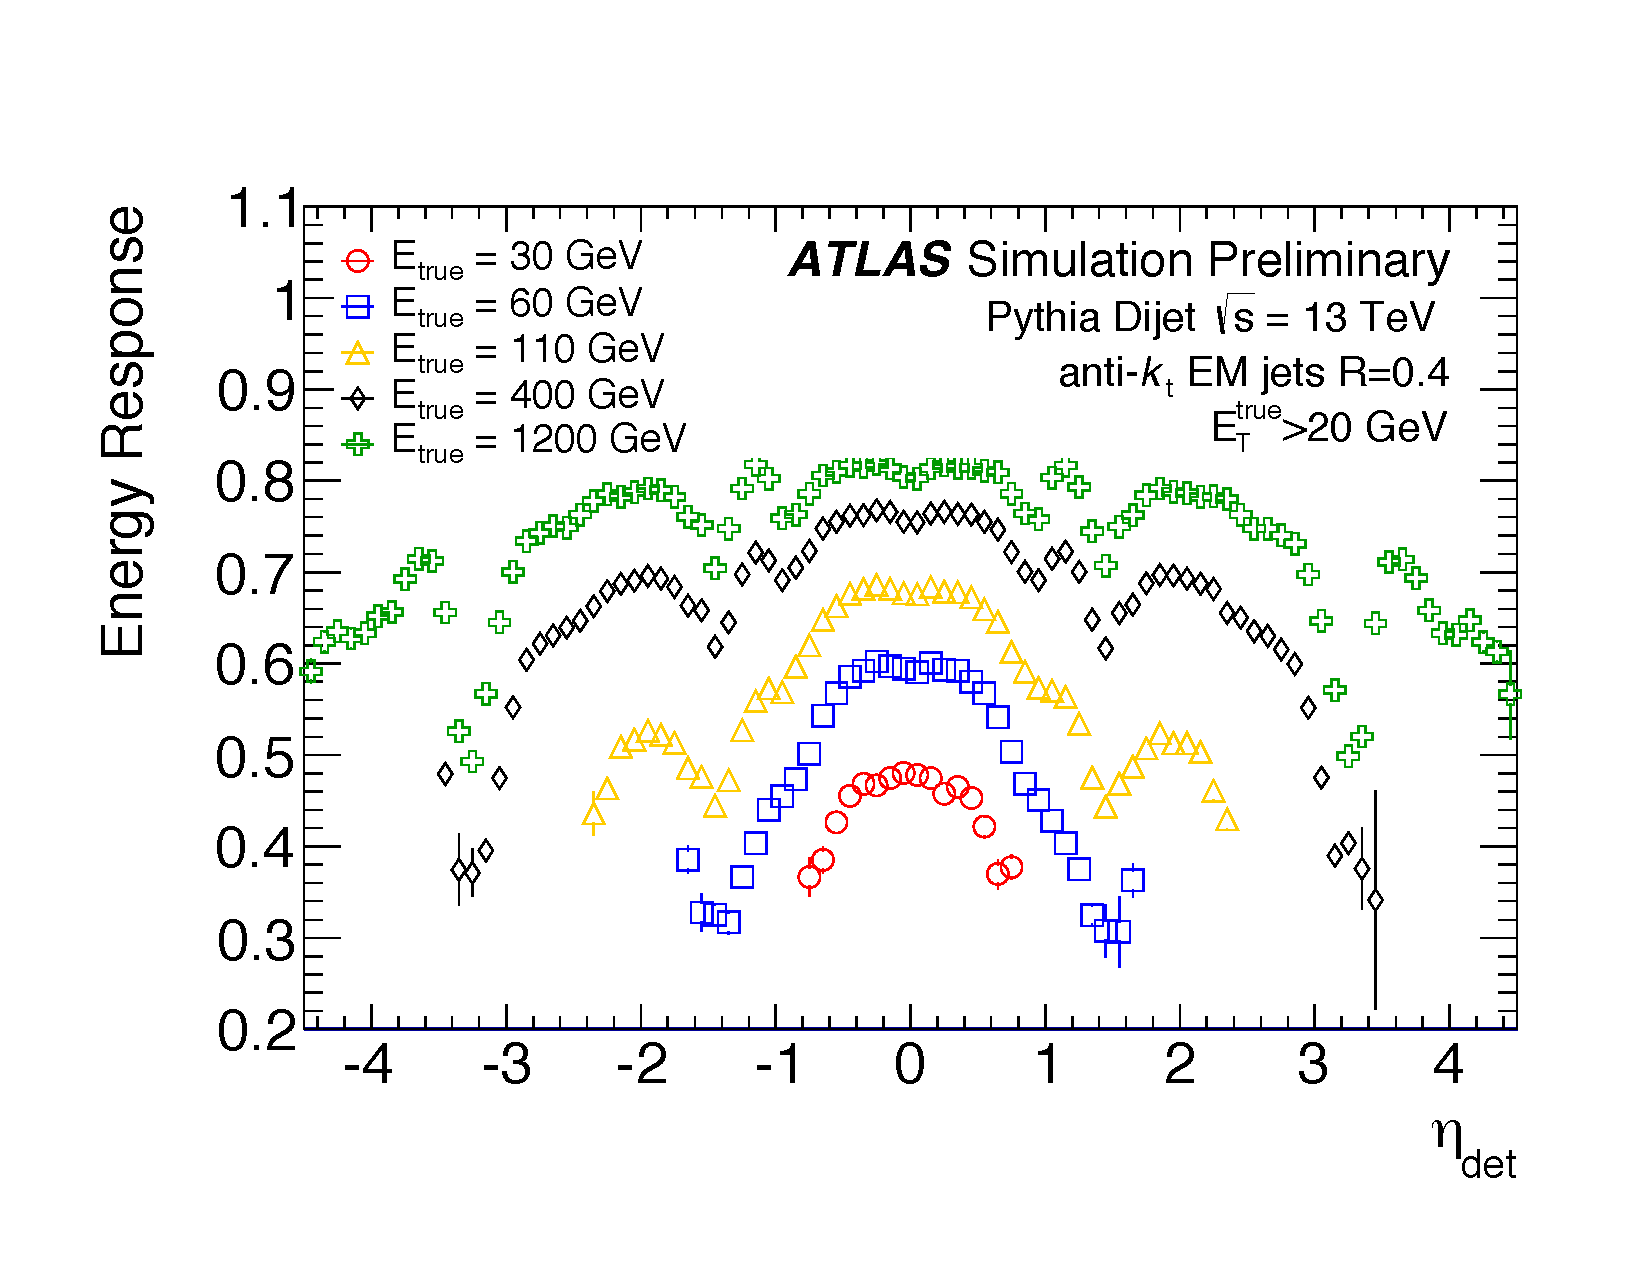
\includegraphics[width=.9\linewidth]{figures/reco/fig_04a.pdf}
\caption{ Energy response as a function of energy and $\eta$ for \ac{EM} jets in dijet \ac{MC}. \cite{ATL-PHYS-PUB-2015-015} }
\label{fig:reco_JES}
\end{figure}
\end{centering}

In addition to correcting for additional energy due to pile-up, it is necessary to reject reconstructed jets that come from pile-up vertices. To accomplish this, a multivariate alogrithm called \ac{JVT} was created which builds upon an older method, \ac{JVF} \cite{ATLAS-CONF-2014-018}. 

\ac{JVF} gives the fraction of energy in a jet that comes from the hard-scatter vertex, and is defined as 
%
\begin{equation}
\mathrm{JVF} = \frac{\sum_i \pt^i(PV_0)}{\sum_j \pt^j(PV_0) + \sum_{n\geq1} \sum_j \pt^j(PV_n)} 
\end{equation}
%
where $\pt^i(PV_n)$ gives the \pt of the $i$th track associated with the $n$th primary vertex. $PV_0$ gives the primary vertex associated with the hard-scattering, while the remaining vertices are due to pile-up interactions. Track are associated with a jet according to a processes called \textit{ghost association}, in which they are clustered along with the typical pseudo-jet collection according to the anti-$k_t$ algorithm described above. In the clustering process, the tracks energy is ignored so that it doesn't impact the measurement of the final jet. 

This fraction decreases with higher pile-up, making the construction of an explicit cut difficult in varying pile-up conditions. \ac{JVT} improved on the method by using a pile-up corrected \ac{JVF}-like variable, defined as 
%
\begin{equation}
\mathrm{corrJVF} = \frac{\sum_i \pt^i(PV_0)}{\sum_j \pt^j(PV_0) + \frac{\sum_{n\geq1} \sum_j \pt^j(PV_n)}{kn_{PU}}} 
\end{equation}
%
where $n_{PU}$ is the number of tracks, which is multiplied by a scaling factor $i = 0.01$. This quantity is included in the inputs of the tagger along with other variables measuring the fraction of jet energy that is associated with the hard-scattering vertex. \autoref{fig:reco_jvt} shows the efficiency and fake rate for the two methods, demonstrating \ac{JVT}'s superior stability across events with different numbers of pile-up vertices. 

\begin{centering}
\begin{figure}[!hbt]
\myfloatalign
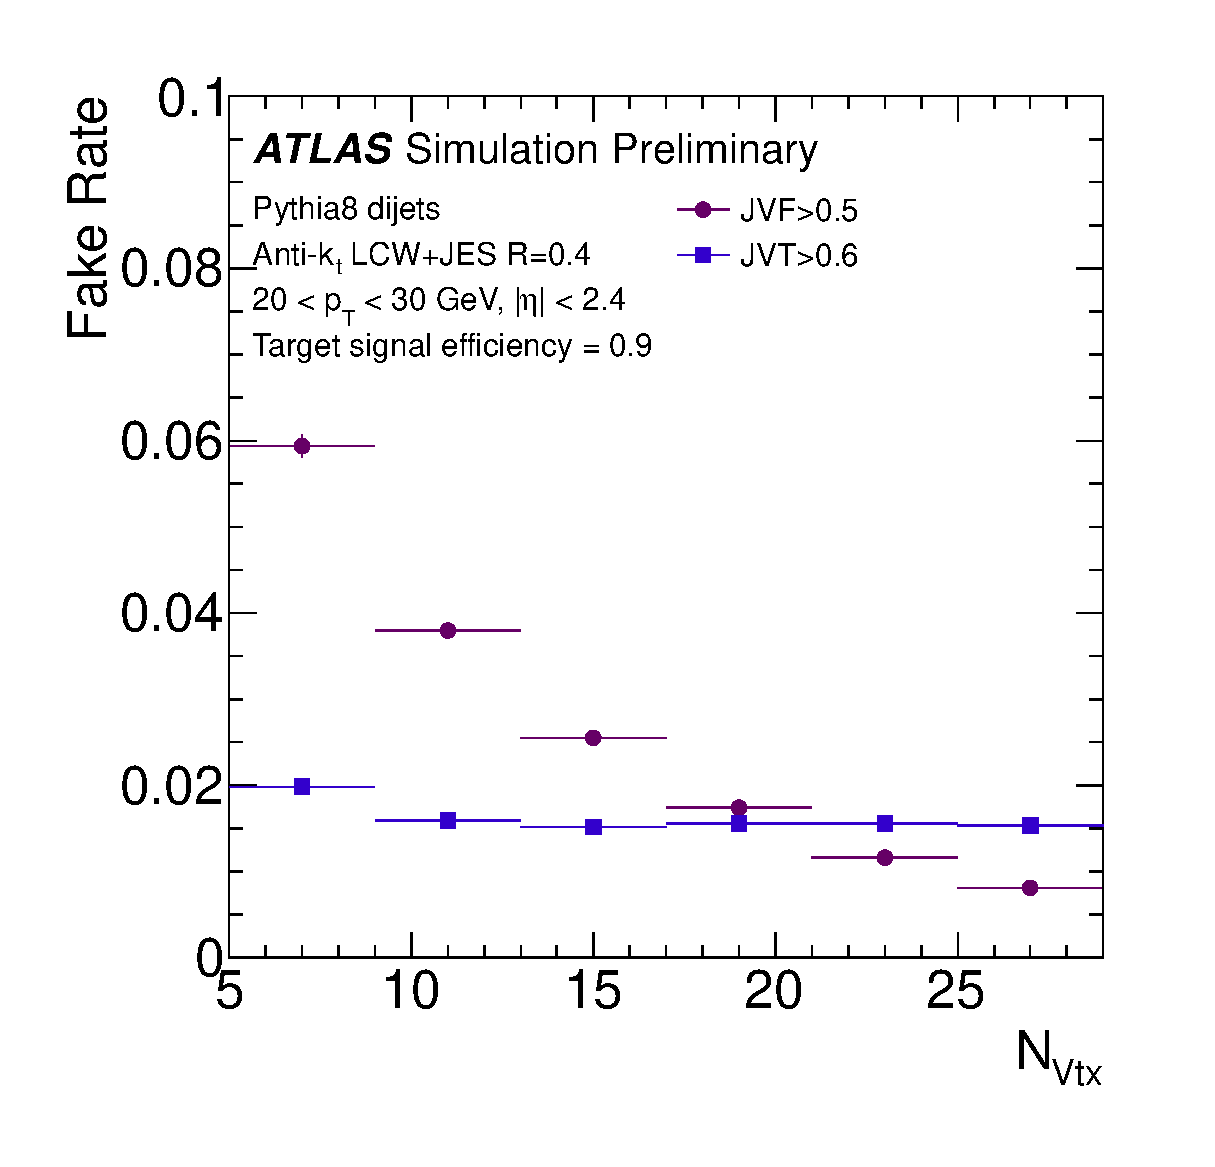
\includegraphics[width=.48\linewidth]{figures/reco/jvt_fig_06b.eps}
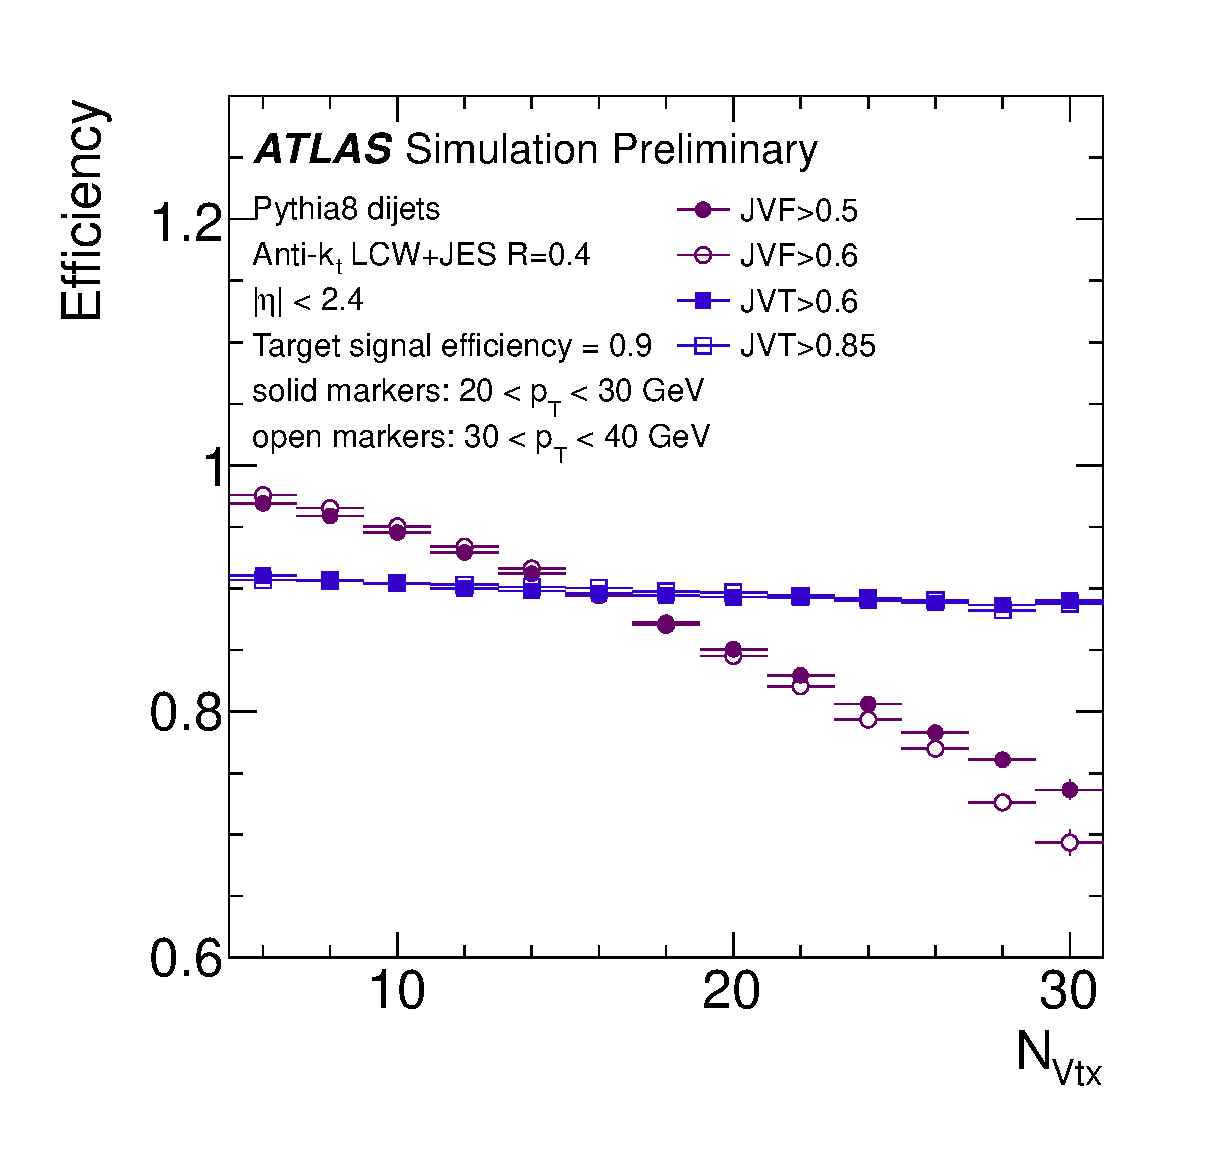
\includegraphics[width=.48\linewidth]{figures/reco/jvt_fig_07a.eps}
\caption{ Dijet \ac{MC} distributions of the number of pile-up jets passing the \ac{JVT} and \ac{JVF} cuts (left) and the efficiency for jets from the primary vertex (right) as a function of number of primary vertices in the event \cite{ATLAS-CONF-2014-018}. }
\label{fig:reco_jvt}
\end{figure}
\end{centering}

It is possible to differentiate jets resulting from $b$-hadron decays from other jets due to the non-negligible lifetimes of the hadrons. Many \ac{BSM} processes preferentially produce $b$ quarks, as do any processes involving top quarks, so this identification can be useful for any analyses seeking to isolate these instances. Multivariate techniques are used to identify secondary vertices using the \ac{ID} \cite{ATL-PHYS-PUB-2015-022}. In \ac{ATLAS}, separate algorithms are used to identify jets with tracks with significantly non-zero impact parameters, tracks that reconstruct a secondary vertex, and tracks that can be identified with a chain of vertices beginning with the primary vertex. This information is fed into a boosted decision tree, a type of multivariate algorithm, called \texttt{MV2c20}, which outputs a discriminant shown in \autoref{fig:reco_mv2}. Using this discriminant, a working point is chosen such that $b$-jets can be identified with a 70\% efficiency, with mis-identification rates at around 12\% for $c$-jets and 0.2\% for light-flavor jets.

\begin{centering}
\begin{figure}[!hbt]
\myfloatalign
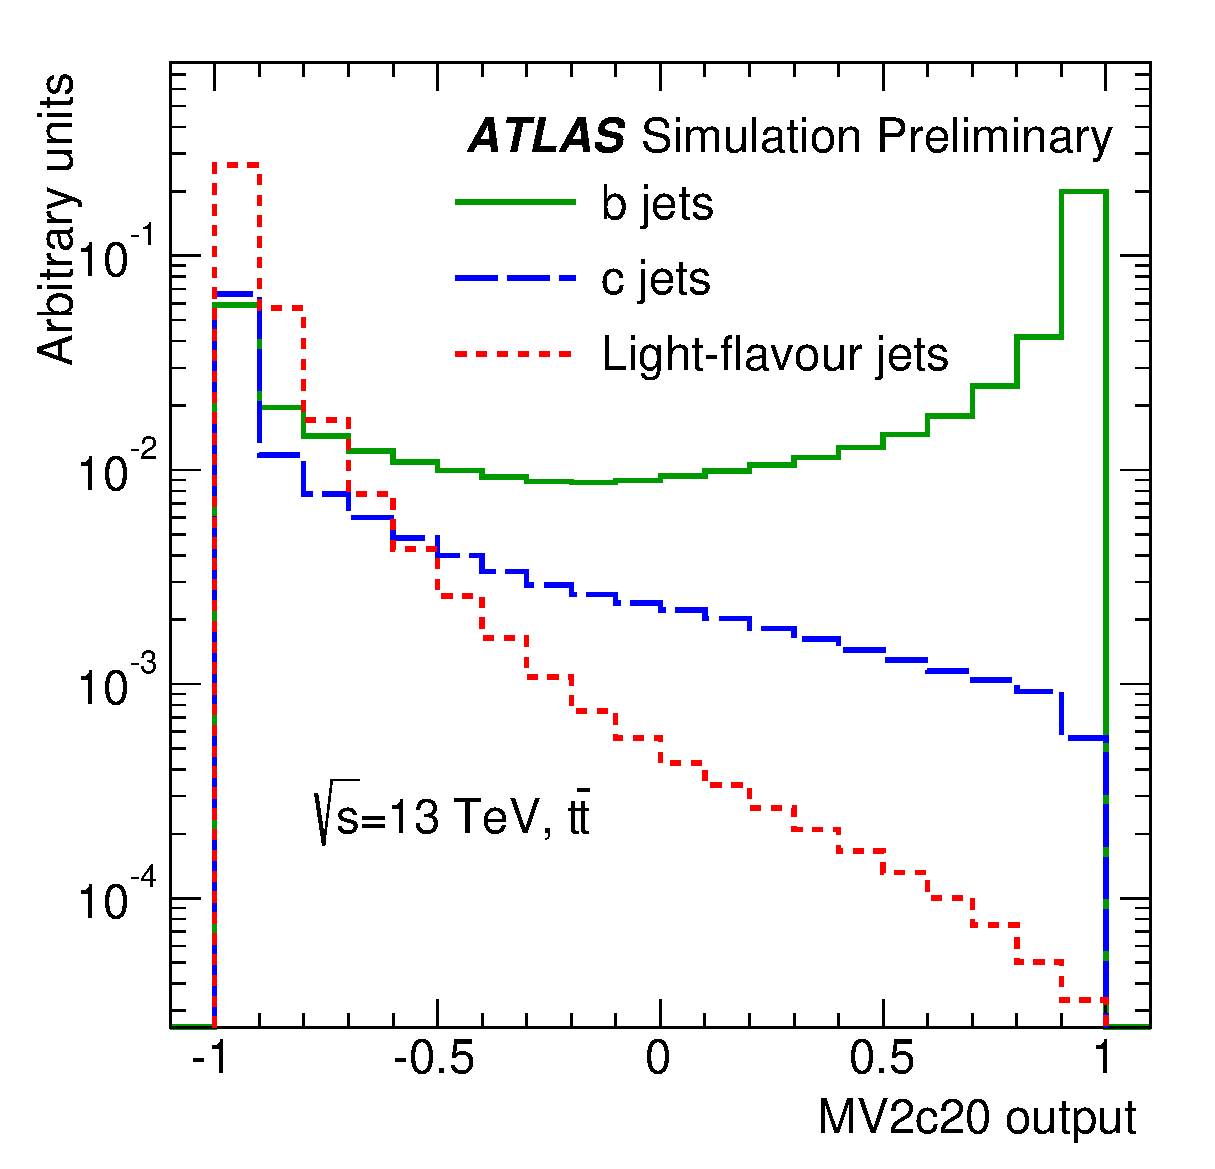
\includegraphics[width=.9\linewidth]{figures/reco/fig_08.eps}
\caption{ Distribution of \texttt{MV2c20} output for $b$-jets, $c$-jets, and light-flavor jets in \ttbar \ac{MC} \cite{ATL-PHYS-PUB-2015-022}. }
\label{fig:reco_mv2}
\end{figure}
\end{centering}

\section{Overlap Removal}
\label{sec:reco_or}

Because most of these reconstruction methods are run independently, it is common for energy deposits and tracks to be shared between jets and particles of different types. To account for this, a process called \acf{OR} is used, which iteratively removes overlapping objects. The process, as well as the calculation of missing transverse momentum described in \autoref{sec:reco_met}, is performed on \textit{baseline} objects. These objects have looser selections than the final \textit{signal} objects, and the separate definitions allow analyzers to tune signal objects to best match a \ac{BSM} signature, while leaving the \ac{OR} process unchanged. The signal and baseline definitions for this analysis are described in \autoref{ch:objects}.

The first step in the \ac{OR} process is to remove reconstructed jets that appear to be due to calorimetric deposits from an electron. To accomplish this, any baseline jet within $\Delta R = 0.2$ from a baseline electron is removed. A caveat is added due to the frequent production of leptons in the decay of heavy-flavor jets; if the jet is $b$-tagged, the electron will be removed instead. After these electrons and jets have been removed, a new search is done for jets and electrons within $\Delta R = 0.4$ of one another. In this iteration, the electron is removed, again to reduce backgrounds from heavy-flavor decays.

Next, the muon-jet \ac{OR} is applied, which is very similar to that of the electron. Any jet within $\Delta R = 0.2$ of a muon is removed, unless the jet is $b$-tagged, in which case the muon is removed due to the likelihood that it resulted due to a heavy-flavor decay. The muon-jet \ac{OR} then differs from the electron's in that a \pt-based $\Delta R$ cut is used in the last step. Muons within $\Delta R < \mathrm{min}(0.04 + (10 \gev)/\pt, 0.4)$ of a jet are removed, with the \pt-dependent cone size designed to reject low-\pt heavy-flavor muons while preserving muons resulting from the decay of high-\pt particles, which are closely aligned with the other products of the decay. 

The next step is to remove electrons likely to have resulted from muon bremsstrahlung. Any electron within $\Delta R = 0.1$ of a muon is removed from the event. 

Lastly, overlap between photons and both jets and electrons is considered. Baseline photons within $\Delta R = 0.4$ of an electron are removed, as are jets within $\Delta R = 0.4$ of a remaining photon.

\section{Missing Transverse Momentum}
\label{sec:reco_met}

Missing transverse momentum (${\boldsymbol p}_{\mathrm{T}}^\mathrm{miss}$, with magnitude \met), is the negative vector sum of \pt measured in an event. Because the colliding protons have no initial transverse momentum, the true value of this quantity should be zero unless a particle escapes the detector without being measured, as neutrinos do. In practice, the reconstructed \met can also be non-zero due to mismeasurement, or due to gaps in the \ac{ATLAS} detector. \met reconstruction is perhaps the most complex because it depends on all other object reconstructions performed in the \ac{ATLAS} detector. 

\met components are calculated independently for each type of baseline object reconstructed, as well as for a soft term, which comprises the energy observed by the \ac{ATLAS} detector but not associated with a baseline object. The soft term can be calculated based either on calorimeter or track measurements \cite{ATL-PHYS-PUB-2015-023}. While the \acf{CST} is very sensitive to pile-up, the \acf{TST} is much more robust, as it excludes tracks emanating from pile-up vertices. Tracks associated with any reconstructed object are also removed. \autoref{fig:reco_met_tst} shows the dependence of the \ac{TST} resolution on number of primary vertices. Because of this lessened pile-up dependence, the \ac{TST} is used to reconstruct \met in this analysis. 

\begin{centering}
\begin{figure}[!hbt]
\myfloatalign
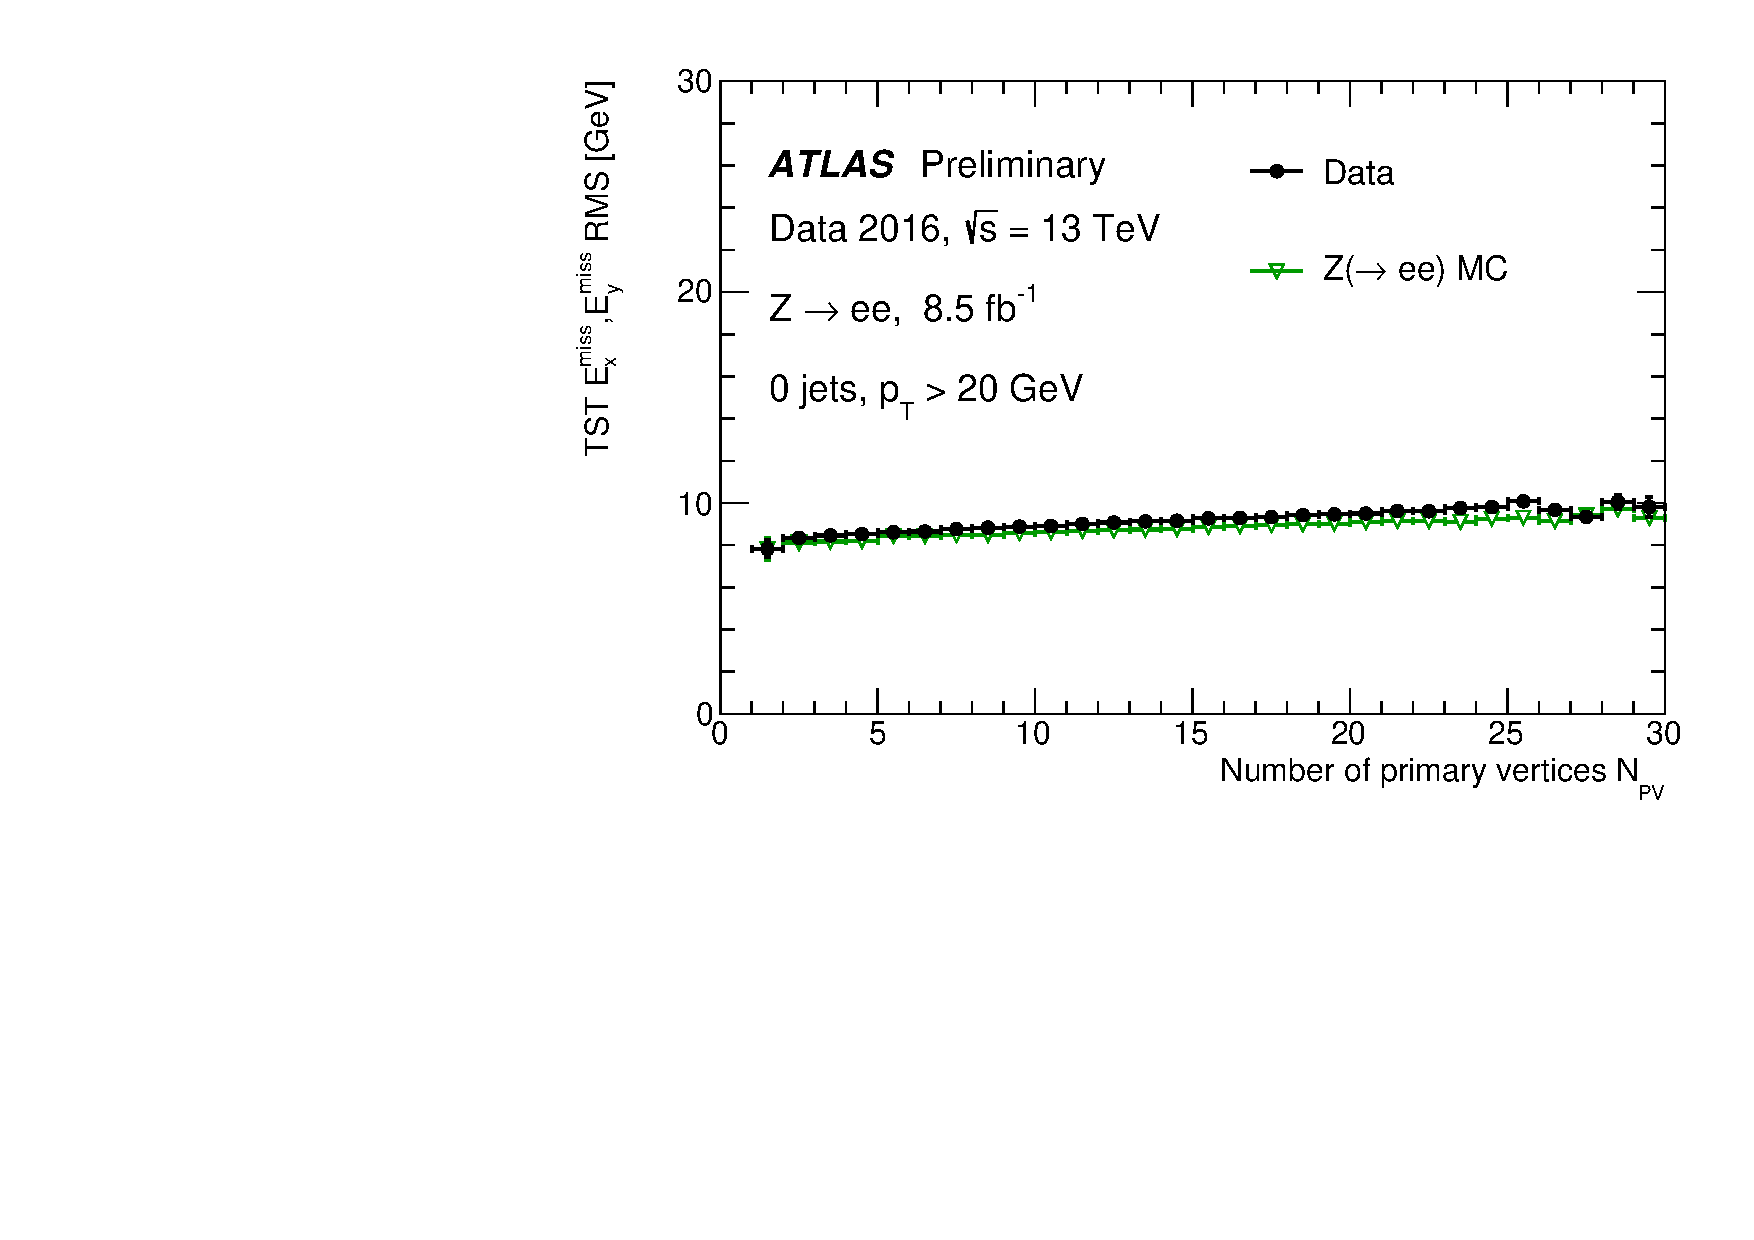
\includegraphics[width=.9\linewidth]{figures/reco/mettst.pdf}
\caption{ Distributions of the resolution of the $x$ and $y$ components of \ac{TST} \met in $Z\rightarrow\mu\mu$ events in data and \ac{MC}. }
\label{fig:reco_met_tst}
\end{figure}
\end{centering}

$Z\rightarrow\mu\mu$ events, which rarely have any true \met, can be used to study the contribution of different objects to the total \met calculation. \autoref{fig:reco_met_terms} shows the the \met resulting from muons, jets, and the soft term measured in events with two opposite-sign muons that reconstruct an invariant mass within 25 \gev~of the $Z$ boson mass. Large values in each of these terms, of course, do not necessarily correspond to a large value of the overall \met; in a system where a $Z$ boson recoils off of a jet system, the terms for jets and muons should both be large but ultimately cancel. However, the overall scale of each term indicates the possibility of contributions from mismeasurement. A 30\% mismeasurement of the jet or muon term can result in significant \met, while a similar mismeasurement of the soft term is unlikely to produce a large impact on the \met calculation. The agreement between data and \ac{MC} in these distributions indicates that, at least in the core of the distributions, these \met terms are well modeled.  

\begin{centering}
\begin{figure}[!hbt]
\myfloatalign
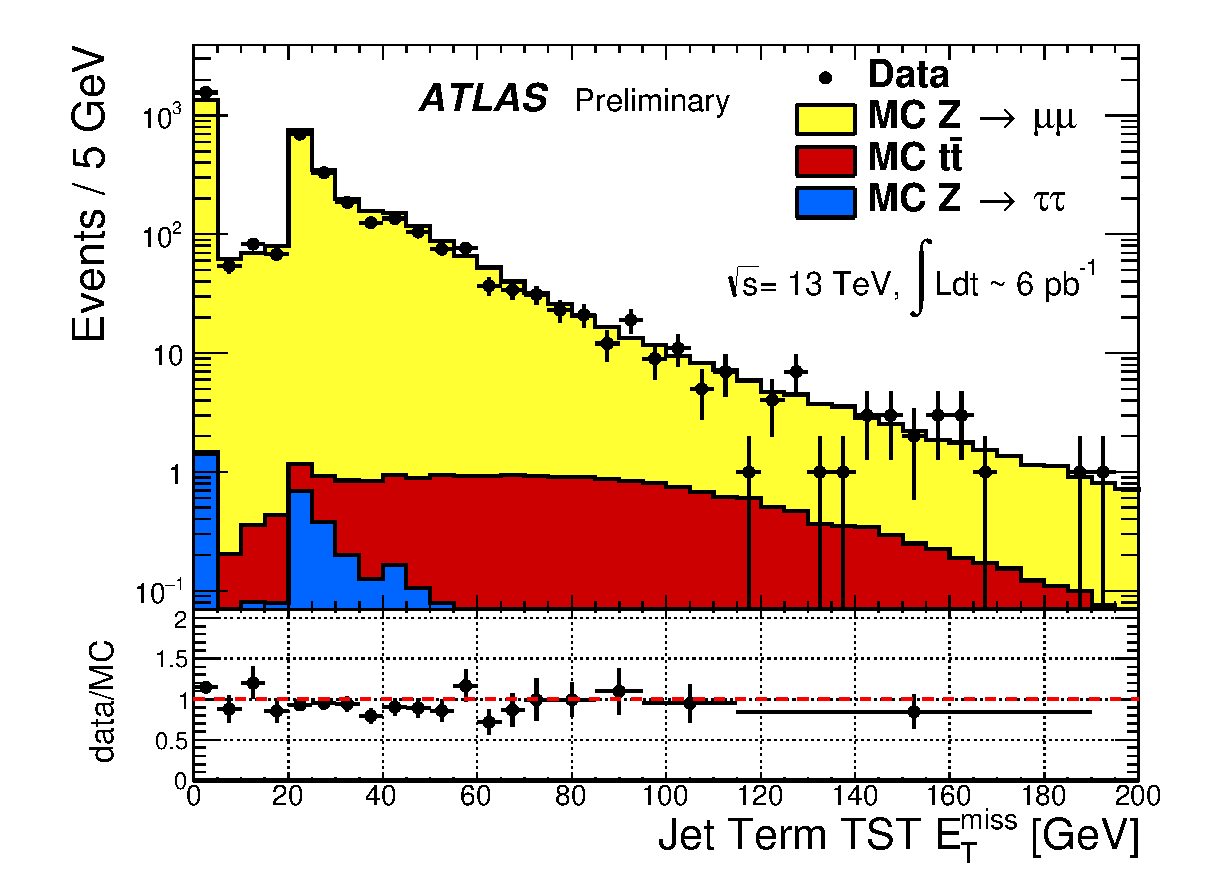
\includegraphics[width=.70\linewidth]{figures/reco/met_fig_02a.eps}
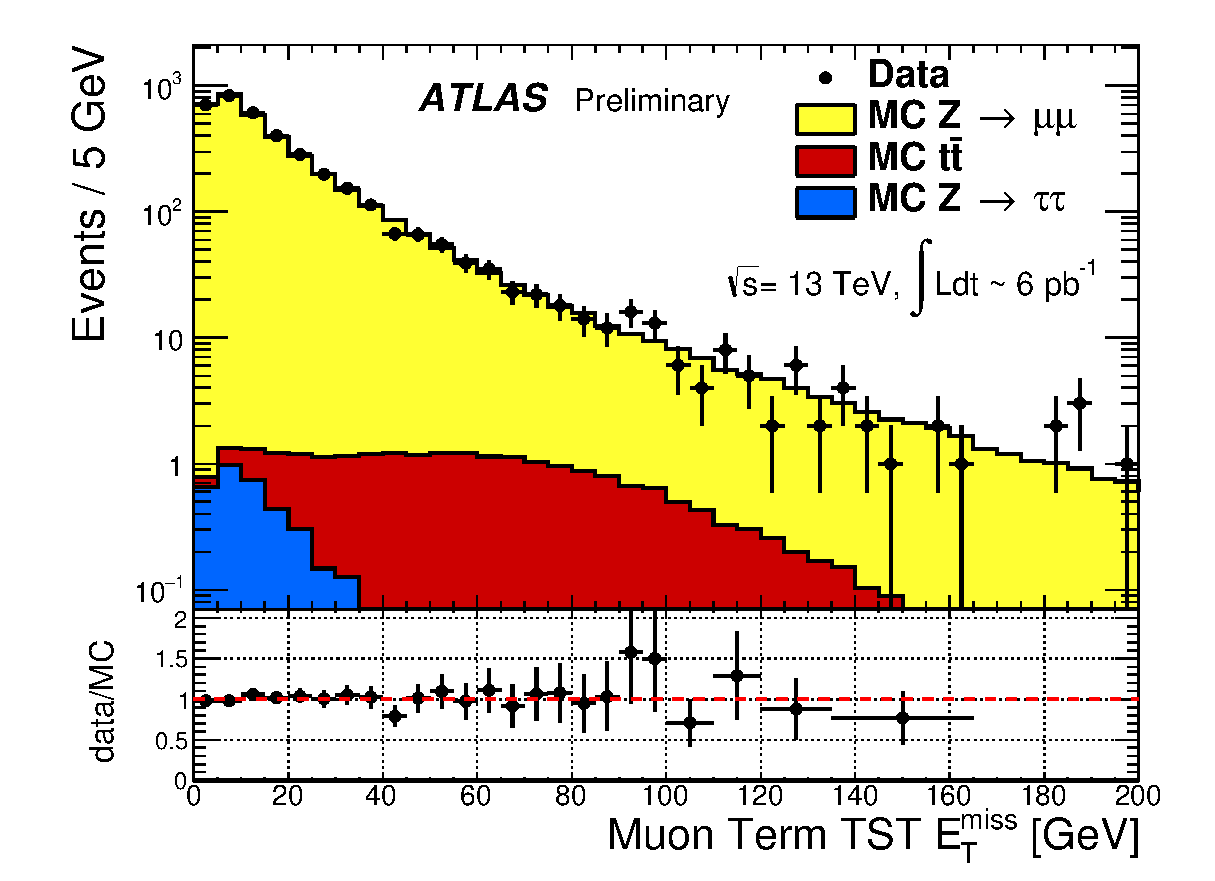
\includegraphics[width=.70\linewidth]{figures/reco/met_fig_02b.eps} \\
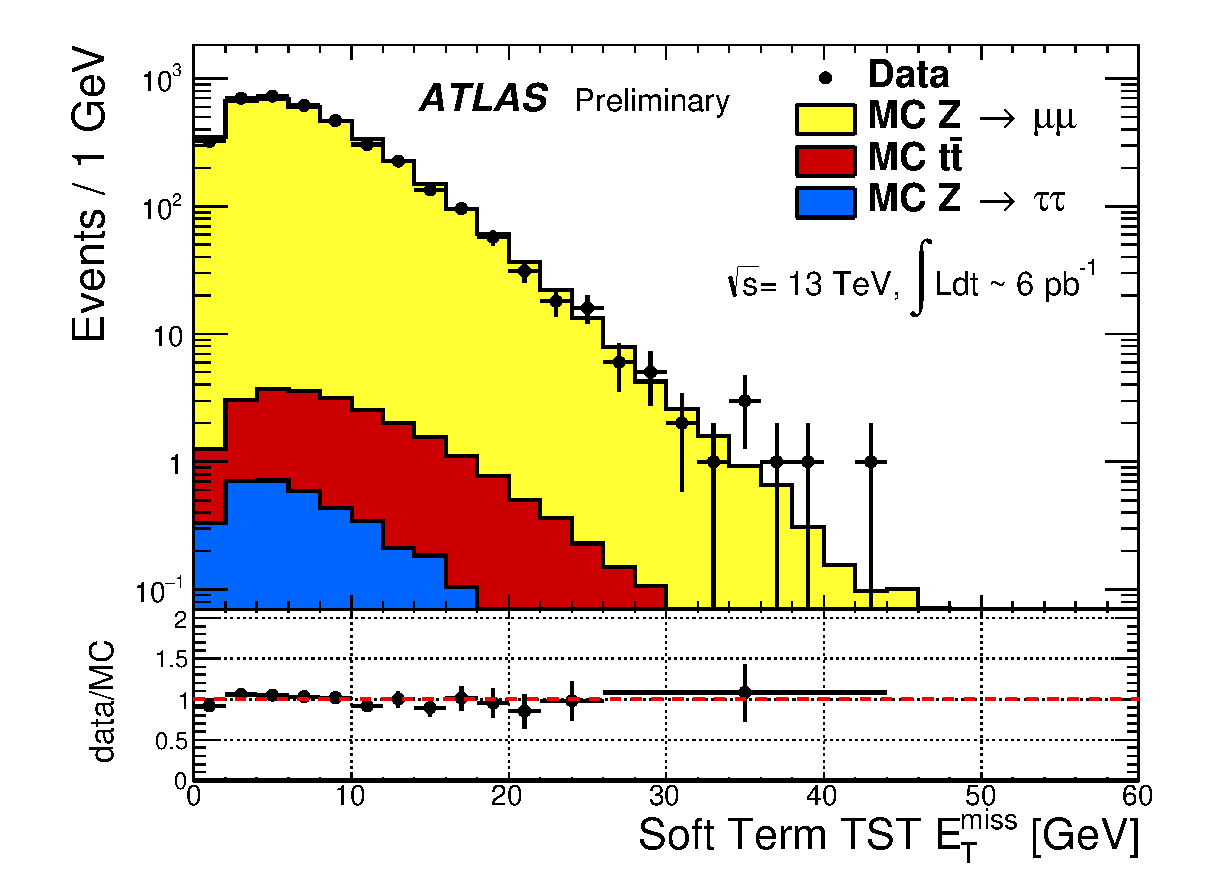
\includegraphics[width=.70\linewidth]{figures/reco/met_fig_02c.eps}
\caption{ Distributions of the jet term (top left), muon term (top right), and \ac{TST} (bottom) \met in $Z\rightarrow\mu\mu$ events in data and \ac{MC}. In the jet term distribution, the feature at zero is due to events with no jets, and the spike at 20 \gev~corresponds to the minimum jet \pt considered for the analysis \cite{ATL-PHYS-PUB-2015-027}. }
\label{fig:reco_met_terms}
\end{figure}
\end{centering}




